\documentclass[twocolumn,twocolappendix,trackchanges]{aastex63}
\usepackage{amsmath}
\newcommand{\code}[1]{\texttt{#1}}
\newcommand{\mesa}{\code{MESA}}
\newcommand{\MESA}{\code{MESA}}
\renewcommand{\labelitemii}{$\bullet$}
\newcommand{\kms}{{\mathrm{km\ s^{-1}}}}
\newcommand{\Msun}{{\mathrm{M}_\odot}}
\newcommand{\kev}{\mathrm{keV}}
\newcommand{\gk}{\ensuremath{\,\rm{GK}}}
\usepackage{CJK}
\DeclareRobustCommand{\Eqref}[1]{Eq.~\ref{#1}}
\DeclareRobustCommand{\Figref}[1]{Fig.~\ref{#1}}
\DeclareRobustCommand{\Tabref}[1]{Tab.~\ref{#1}}
\DeclareRobustCommand{\Secref}[1]{Sec.~\ref{#1}}
\newcommand{\zoph}{$\zeta$ Oph}

\newcommand{\todo}[1]{{\large $\blacksquare$~\textbf{\color{red}[#1]}}~$\blacksquare$}

\defcitealias{villamariz:05}{VH05}


\begin{document}

\graphicspath{{./figures/}}


\title{Accretor stars in massive binaries: testing models on  $\zeta$ Ophiuchi}

\author[0000-0002-6718-9472]{M.~Renzo}
\affiliation{Department of Physics, Columbia University, New York, NY 10027, USA}
\affiliation{Center for Computational Astrophysics, Flatiron Institute, New York, NY 10010, USA}

\author[0000-0002-6960-6911]{Y.~G\"otberg}
\affiliation{The Observatories of the Carnegie Institution for Science, 813 Santa Barbara Street, Pasadena, CA 91101, USA}


\begin{abstract}
  Most massive stars are born in binary systems close enough
  for mass-transfer episodes. These modify the appearance, internal
  structure, and future evolution of both stars. However,
  models of the accretors are rare.  The nearest
  O-type star to Earth, $\zeta$ Ophiuchi, has long been
  proposed to have accreted mass from a former companion, before being
  ejected as a runaway by the companion's supernova
  explosion. Therefore, this star provides an ideal test bed for
  models of accretors in binaries. We use % the open-source stellar
  % evolution code
  \texttt{MESA} to model the evolution of a massive binary (initially
  $M_1=25\,M_\odot$, $M_2=17\,M_\odot$) evolving through a stable mass
  transfer after the donor's main sequence (case B, initial period
  100\,days). Adopting common assumptions for the treatment of
  rotation, chemical mixing, and mass transfer, our accreting star
  reproduces reasonably well the kinematic, spectroscopic, and
  photometric properties of $\zeta$ Ophiuchi. We compare our accretor
  to fast-rotating single stars: the late spin-up through
  mass transfer causes the accretor core to spin faster at the end of
  the main sequence, and the rejuvenation causes an off-center
  convective layer which impacts the density structure at the envelope base.
  Our models demonstrate the impact of
  mass accretion on the secondary star in a binary, with possible
  implications for its further evolution (either in a binary or as
  single stars), the final collapse, and the resulting spins of the
  compact object formed.
\end{abstract}

\vspace*{-10pt}
\keywords{stars: individual: $\zeta$ Ophiuchi  -- stars: massive --
  stars: binaries} %% check keywords exist

\section{Introduction}
\label{sec:intro}


The overwhelming majority of massive stars is born in multiple systems
\citep[e.g.,][]{mason:09, almeida:17, moe:17}, and a large fraction will
exchange mass or merge with a companion in their lifetime
\citep[e.g.,][]{sana:12}. The most common type of interaction is a
stable mass transfer through Roche Lobe overflow (RLOF) after the end of the donor's main sequence (case
B, \citealt{kippenhahn:67}).  Many
studies %\todo{more refs. from other groups}
have focused on the dramatic impact these interactions have on the
donor star \citep[e.g.,][]{morton:60, yoon:17, gotberg:17, gotberg:18, laplace:20,
  laplace:21, blagorodnova:21}. Often the accreting companion is treated as a point mass.
However, binary interactions have a crucial impact on the initially
less massive star too.

\subsection{The importance of accretor stars}

During mass transfer, the initially less massive star is expected to
accrete mass, spin-up to critical rotation \citep[e.g.,][]{packet:81},
and possibly be polluted by nuclearly processed material from the
inner core of the donor star \citep[e.g.,][]{blaauw:93}. The growth of
the convective core due to the increased mass leads to
``rejuvenation'' of the accretor \citep[e.g.,][]{neo:77,
  schneider:16}. Understanding the evolution of accretors in massive
binaries has wide and crucial implications for stellar populations,
electromagnetic transient observations, and gravitational-wave
progenitors.

Accretors
(and merger products) can appear as blue stragglers
\citep[e.g.,][]{chen:09, chen:10, rain:21} and thus impact cluster
populations, their age estimates, and their main sequence
\citep[e.g.,][]{pols_marinus:94, wang:20} and post main sequence morphology
\citep[e.g.,][]{wei:21}. The high spin of the
accretor post-mass-transfer might be the dominant explanation for the origin of
Oe and Be stars \citep[i.e., stars showing emission lines, e.g.,][]{pols:91, bodensteiner:20,
  vinciguerra:20, dorigo-jones:20, wang:21_sdOBe}. Rotationally-mixed accreting
stars at low metallicity might also be important for the ionizing flux of high-redshift
galaxies \citep[e.g.,][]{eldridge:12}.

After mass transfer, the majority of massive binaries will be
disrupted by the first supernova, and eject the accretor \citep[``binary SN
scenario'', ][]{blaauw:61, dedonder:97, eldridge:11, boubert:18,
  renzo:19walk, evans:20}.  A small fraction of these would be
sufficiently fast to become runaway stars, but the majority will be
too slow to stand out in astrometric surveys. Assuming a constant star
formation history, \cite{renzo:19walk} estimated that
$10.1^{+4.6}_{-8.6}\%$ ($0.5^{+2.1}_{-0.5}\%$) of O-type stars could
be slow ``walkaway'' (runaway) accretors ejected after the companion's
SN explosion.  Therefore, presently single O-type stars that accreted
mass earlier on contribute to the populations of field massive stars.

From the transients perspective, massive accretor stars are also
important: \cite{zapartas:19} estimated that $14_{-11}^{+4}\%$ of
hydrogen (H) rich
type II SNe might come from progenitors ejected from a binary after
the explosion of their companion. The fact that they accreted mass before exploding can
influence their helium (He) core mass and thus the explosion
properties and the inferred progenitors \citep{zapartas:21}. % Some
% stars might not have been massive enough to reach core-collapse
% without accreting mass from a companion
% \citep[e.g.,][]{zapartas:17}. The number of accretors is tiny, those
% are mergers for the vast part
The high post-mass transfer rotation
rate of accretor stars in binaries might have implications for the
formation of long gamma-ray burst progenitors \citep[e.g.,][]{cantiello:07}.

Finally, the majority of isolated binary evolution scenarios for
gravitational-wave progenitors include a common-envelope
phase. This is initiated by the originally less massive star, who
accretes mass from its companion before the formation of the first compact object
\citep[e.g.,][]{belczynski:16nat, tauris:17,
  broekgaarden:21}. Therefore, it is possible that accretion of mass
before the formation of the first compact object could modify the
internal structure of the star that will initiate the common-envelope
\citep[e.g.,][]{law-smith:20, klencki:21}. Specifically, the
rotation rate, chemical composition, and innermost structure of the
envelope (because of rejuvenation) might differ from a single star.

Despite their importance, accretor stars in binaries have so far
received much less attention than the donor stars, with the pioneering
studies of \cite{ulrich:76, hellings:83, hellings:84}, and
\cite{braun:95} as notable exceptions. Large grids of accretor models
are lacking, most of the studies focus on lower mass systems
(e.g., $M_1\lesssim 16\,M_\odot$ in \citealt{vanrensbergen:11}) or
neglect the crucial impact of rotation (e.g., \citealt{sravan:19}, but see also
\citealt{wang:20}) and only few sparse massive models exist
\citep[e.g.,][]{cantiello:07}.

Modeling accretor stars requires following the coupled evolution of
two rotating stars exchanging mass. Making robust predictions is
challenging because of the admittedly large number of free parameters
necessary to model each individual star and their interactions. Rapid
population synthesis typically cannot include the effects of binary
mass transfer on the internal structure of the stars, and rely on the
implicit assumption that the accretor is sufficiently well described
by a (possibly fast-rotating) single star model. Here, we compute
detailed evolutionary models of both stars in a binary and compare our
accretor to rotating single star models to test this assumption.

\subsection{A prototypical example of accretor: $\zeta$ Ophiuchi}

The nearest O-type star to Earth, $\zeta$
Ophiuchi\footnote{also known as HD\,149\,757.} (\zoph) provides a
unique opportunity to constrain massive binary evolution models.  \zoph\ has a distance
from Earth of $107\pm4$\,pc \citep[][and references
therein]{neuhauser:20}, and a spectral type O9.5{\rm IVnn}
\citep{sota:14}. It occasionally shows emission lines, making it an Oe
star \citep{walker:79, vink:09}. Its surface rotation rate is
extremely large, with most estimates of the projected rotational
velocity from optical spectra exceeding $v\sin(i)\gtrsim 400\,\kms$
(corresponding to the ``nn'' in the spectral type, \citealt{zehe:18}
and references therein). By comparing the
observed $v\sin(i)=432\pm16\,\kms$ to the theoretical breakup
rotation, \cite{zehe:18} constrained the inclination angle to
$i\gtrsim 56$\,degrees. Using optical interferometry, \cite{gordon:18}
were able to measure the centrifugal distorsion of \zoph, and found a
polar radius of $7.5\,R_\odot$ and centrifugally increased equatorial
radius of $9.1\,R_\odot$, corresponding to a $v\sin(i)=348\,\kms$.

\zoph\ was originally
identified as a runaway because of its large proper motion by
\cite{blaauw:52}. Unfortunately, the \emph{Gaia} data for this object
are not of sufficient quality\footnote{The renormalized unit weighted
  error (RUWE) of this star in Gaia EDR3 is 4.48.} to improve previous astrometric results,
but estimates of the peculiar velocity range in $30-50\,\kms$
\citep[e.g.,][]{zehe:18, neuhauser:20}. The large velocity with
respect the surrounding interstellar material is also confirmed by the
presence of a prominent bow-shock \citep[e.g.,][]{bodensteiner:18}.

Because of its young apparent age, extremely fast rotation, and nitrogen
(N) and He rich surface \citep[e.g.,][]{herrero:92, blaauw:93,
  villamariz:05, marcolino:09}, \zoph\ is a prime example of runaway from the binary SN scenario \citep{blaauw:93}. Many studies have suggested
\zoph\ might have accreted mass from a companion before acquiring its
large velocity, both from spectroscopic and kinematic considerations
\citep[e.g.,][]{blaauw:93, hoogerwerf:00, hoogerwerf:01, tetzlaff:10,
  neuhauser:20} and using stellar modeling arguments
\citep[e.g.,][]{vanrensbergen:96}. Recently, \cite{neuhauser:20}
suggested that $1.78\pm0.21$\,Myr ago a SN in
Upper-Centaurus-Lupus produced the pulsar PSR B1706-16, ejected \zoph,
and also injected the short-lived radioactive isotope
$^{60}\mathrm{Fe}$ on Earth. This argues strongly for a successful
SN explosion of the companion with a $\sim 250\,\kms$ natal
kick, sufficient in most cases to disrupt the binary
\citep[e.g.,][]{tauris:15, renzo:19walk, evans:20}.

Although the nature of \zoph\ as a binary product is well established,
because of its observed large surface rotation rate, previous attempts
to model it rely purely on rotational mixing to explain the N- and
He-rich surface composition \cite[e.g.,][]{maeder:00}. Even the binary
models of \cite{vanrensbergen:96} assumed rotational mixing from the
inside of the accreting star driven by the spin-up during mass
transfer (see also \citealt{cantiello:07}). However, \cite{villamariz:05}
(hereafter, \citetalias{villamariz:05}) were unable to find good fit
for the stellar spectra using the single-star rotating models from
\cite{meynet:00, meynet:03}: by the time rotational mixing enriches
the surface, single massive stars have significantly spin down through
wind mass loss.

This may not be surprising: algorithms modeling rotational mixing
predict lower efficiency for metal-rich and relatively low mass
stars. The reason is the increased importance of mean molecular weight
gradients and the longer thermal timescales compared to more massive
stars \citep[e.g.,][]{yoon:06, perna:14}. The parent association of
\zoph\ has a metallicity $Z=0.01\simeq Z_\odot$ \citep[based on
asteroseismology from][]{murphy:21}, and mass estimates for \zoph\
range from $13-25\,M_\odot$, at the lower end of the range where
rotational mixing can efficiently bring He and CNO-processed material to the
surface (chemically homogeneous evolution, \citealt{maeder:00}).

Given the challenges in explaining the surface composition of \zoph\
as a rotating single star and the evidence for its past as a member of
a binary system, this star offers a unique opportunity to constrain
the evolution of accretors in massive binaries.
Here, we present self-consistent binary evolution models for
$\zeta$ Oph computing simultaneously the coupled evolution of
\emph{both} donor and accretor star and their orbit. After describing
our \texttt{MESA} setup in \Secref{sec:methods}, we show our best model which
reproduces the majority of the salient features of this star in
\Secref{sec:best_model}. %  In this model, the surface abundances of
% \zoph\ are explained by pollution from the former companion, rather
% than upward mixing from the interior of \zoph\ itself.
We discuss the
sensitivity of our results to the admittedly many free parameters
% required for this kind of computations
in
\Secref{sec:discussion}, before concluding in
\Secref{sec:conclusions}.



\section{Modeling massive binaries with \texttt{MESA}}
\label{sec:methods}

Modeling the evolution of massive binaries
($M_1\gtrsim 20\,M_\odot \geq M_2$) is challenging because of the
intricate role of several notoriously difficult stellar physics
ingredients (accretion, differential rotation, mixing, high mass-loss
rates, etc.). We follow self-consistently the coupled evolution
of two massive stars in a binary system using \texttt{MESA} (version
15140, \citealt{paxton:11, paxton:13, paxton:15, paxton:18,
  paxton:19}). Our choice of input parameters and our numerical
results are available at \todo{zenodo}. We discuss here
only the main relevant physical parameters and describe tests changing
some of the fiducial values in
\Secref{sec:discussion}. Appendix~\ref{sec:software} gives more
details on our choice of input physics, and
appendix~\ref{sec:res_tests} discuss the numerical resolution in space
and time.

We adopt the \cite{ledoux:47} criterion to determine convective
stability and a mixing length parameter of $1.5$. We allow for
time-dependent convection as in \cite{renzo:20:ppi_conv} based on
\cite{arnett:69}. We include semiconvection and thermohaline mixing
following \cite{langer:83} and \cite{kippenhahn:80}, respectively,
each with efficiency $1.0$. We use the exponential core overshooting
from \cite{herwig:00} with free parameters
$(f, f_0)=(4.25\times10^{-2}, 10^{-3})$ \citep{claret:17} which
broadly reproduce the width of the main sequence from
\cite{brott:11}. We do not use over/undershooting for off-center
convective shells. We also use the local implicit enhancement of the
convective flux in superadiabatic regions introduced
in \texttt{MESA} 15140.

We treat rotation in the ``shellular'' approximation
\citep[e.g.,][]{zahn:92, ekstrom:12}, that is we
assume constant rotational frequency $\omega$ along isobaric
surfaces. Furthermore, we assume tidal synchronization and rigid
rotation at zero age
main sequence (ZAMS) -- the beginning of our runs. For our fiducial
period of $P=100$\,days, this means the stars are initially slow
rotators: the surface averaged rotational velocity is
$\lesssim3\,\kms$ for both. Our models include a diffusive
approximation for meridional currents (Eddington-Sweet circulations, \citealt{sweet:50}), which
dominate the chemical mixing due to rotation. We also include the
secular and dynamical shear instabilities, and the
Goldreich-Schubert-Fricke (GSF) instability.  We assume a Spruit-Tayler
dynamo for the transport of angular momentum \citep{spruit:02}, and
chose the same free parameters as \cite{heger:00}. This also includes
the implicit rotational enhancement of wind mass loss to keep the
rotation sub-critical as in \cite{langer:98}. Specifically, at each
timestep we calculate a wind enhancement factor to reduce the ratio
$\omega/\omega_\mathrm{crit}\lesssim 0.95$ where
$\omega_\mathrm{crit}=\sqrt{(1-L/L_\mathrm{Edd})GM/R^3}$ and
$L_\mathrm{Edd}$ is the Eddington luminosity computed using the
stellar opacity down to optical depth
$\tau=2/3$, $L$ is the luminosity, $R$ the radius, and $G$
the gravitational constant. However, we allow a tolerance of 0.05 on
this limit.



We assume a fiducial metallicity of $Z=0.01$ informed by the
present-day $Z$ of \zoph's parent cluster \citep{murphy:21}, and assume
the relative element abundances to scale with solar values \citep{grevesse:98}. We include wind mass loss following
\cite{vink:00,vink:01} for effective
temperature $T_\mathrm{eff}\gtrsim10^{4.2}$\,K, and \cite{dejager:88} for  $T_\mathrm{eff}\lesssim10^{4.2}$\,K, both with a scaling
factor of 1. Nominally, this means our wind mass-loss rate post-mass
transfer is overestimated by about a factor of 100 compared to
observations \citep[weak wind problem, see][]{marcolino:09}.  However,
\cite{lucy:12} and \cite{lagae:21} proposed that the temperature
structure of the winds of low-luminosity O-type stars might affect the
spectral lines and cause an empirical underestimate of the mass-loss
rate.

Both stars are evolved simultaneously on the same timesteps until
after the donor detaches from its Roche lobe. We follow \cite{kolb:90}
to calculate with an implicit scheme the mass transfer rate. Moreover, we
assume that the specific angular momentum and entropy of the
transferred layers match the surface of the accretor, while the chemical composition
is set by the stratification of the donor star. Mass transfer is
conservative until the accretor reaches critical rotation, after which
rotationally-enhanced mass loss governs the mass transfer efficiency.
Transferred matter which is not successfully accreted carries away the
specific angular momentum corresponding to the accretor's orbital
motion.


% To define RLOF detachment, we take advantage of the fact that we focus
% here on case B interactions among massive stars.
After losing their envelopes, massive donors are not expected to
expand to hundreds of $R_\odot$ during He-shell burning at the
metallicity we consider (e.g., \citealt{laplace:20}, however see also
\citealt{gilkis:19}). Thus, we stop evolving a binary system when the
donor's surface He mass fraction is larger than 0.35 -- indicating
that a significant amount of envelope has been lost or transferred,
and the radius is smaller than both the Roche radius and the
terminal-age main sequence radius (TAMS, defined as when the central
mass fraction of H drops below $10^{-4}$). From here
onwards, % At this point in time,
% we save a model for the accreting star, and continue its evolution
% as
we continue the evolution of the accretor as a single star until its TAMS
with the same setup.

%repetition
% We discuss some parameter variations for the physics of each star, the
% initial conditions, and the binary interactions in \Secref{sec:discussion}.

\section{Massive binary evolution naturally explains $\zeta$
  Ophiuchi's properties}
\label{sec:best_model}

\begin{figure}[tp]
  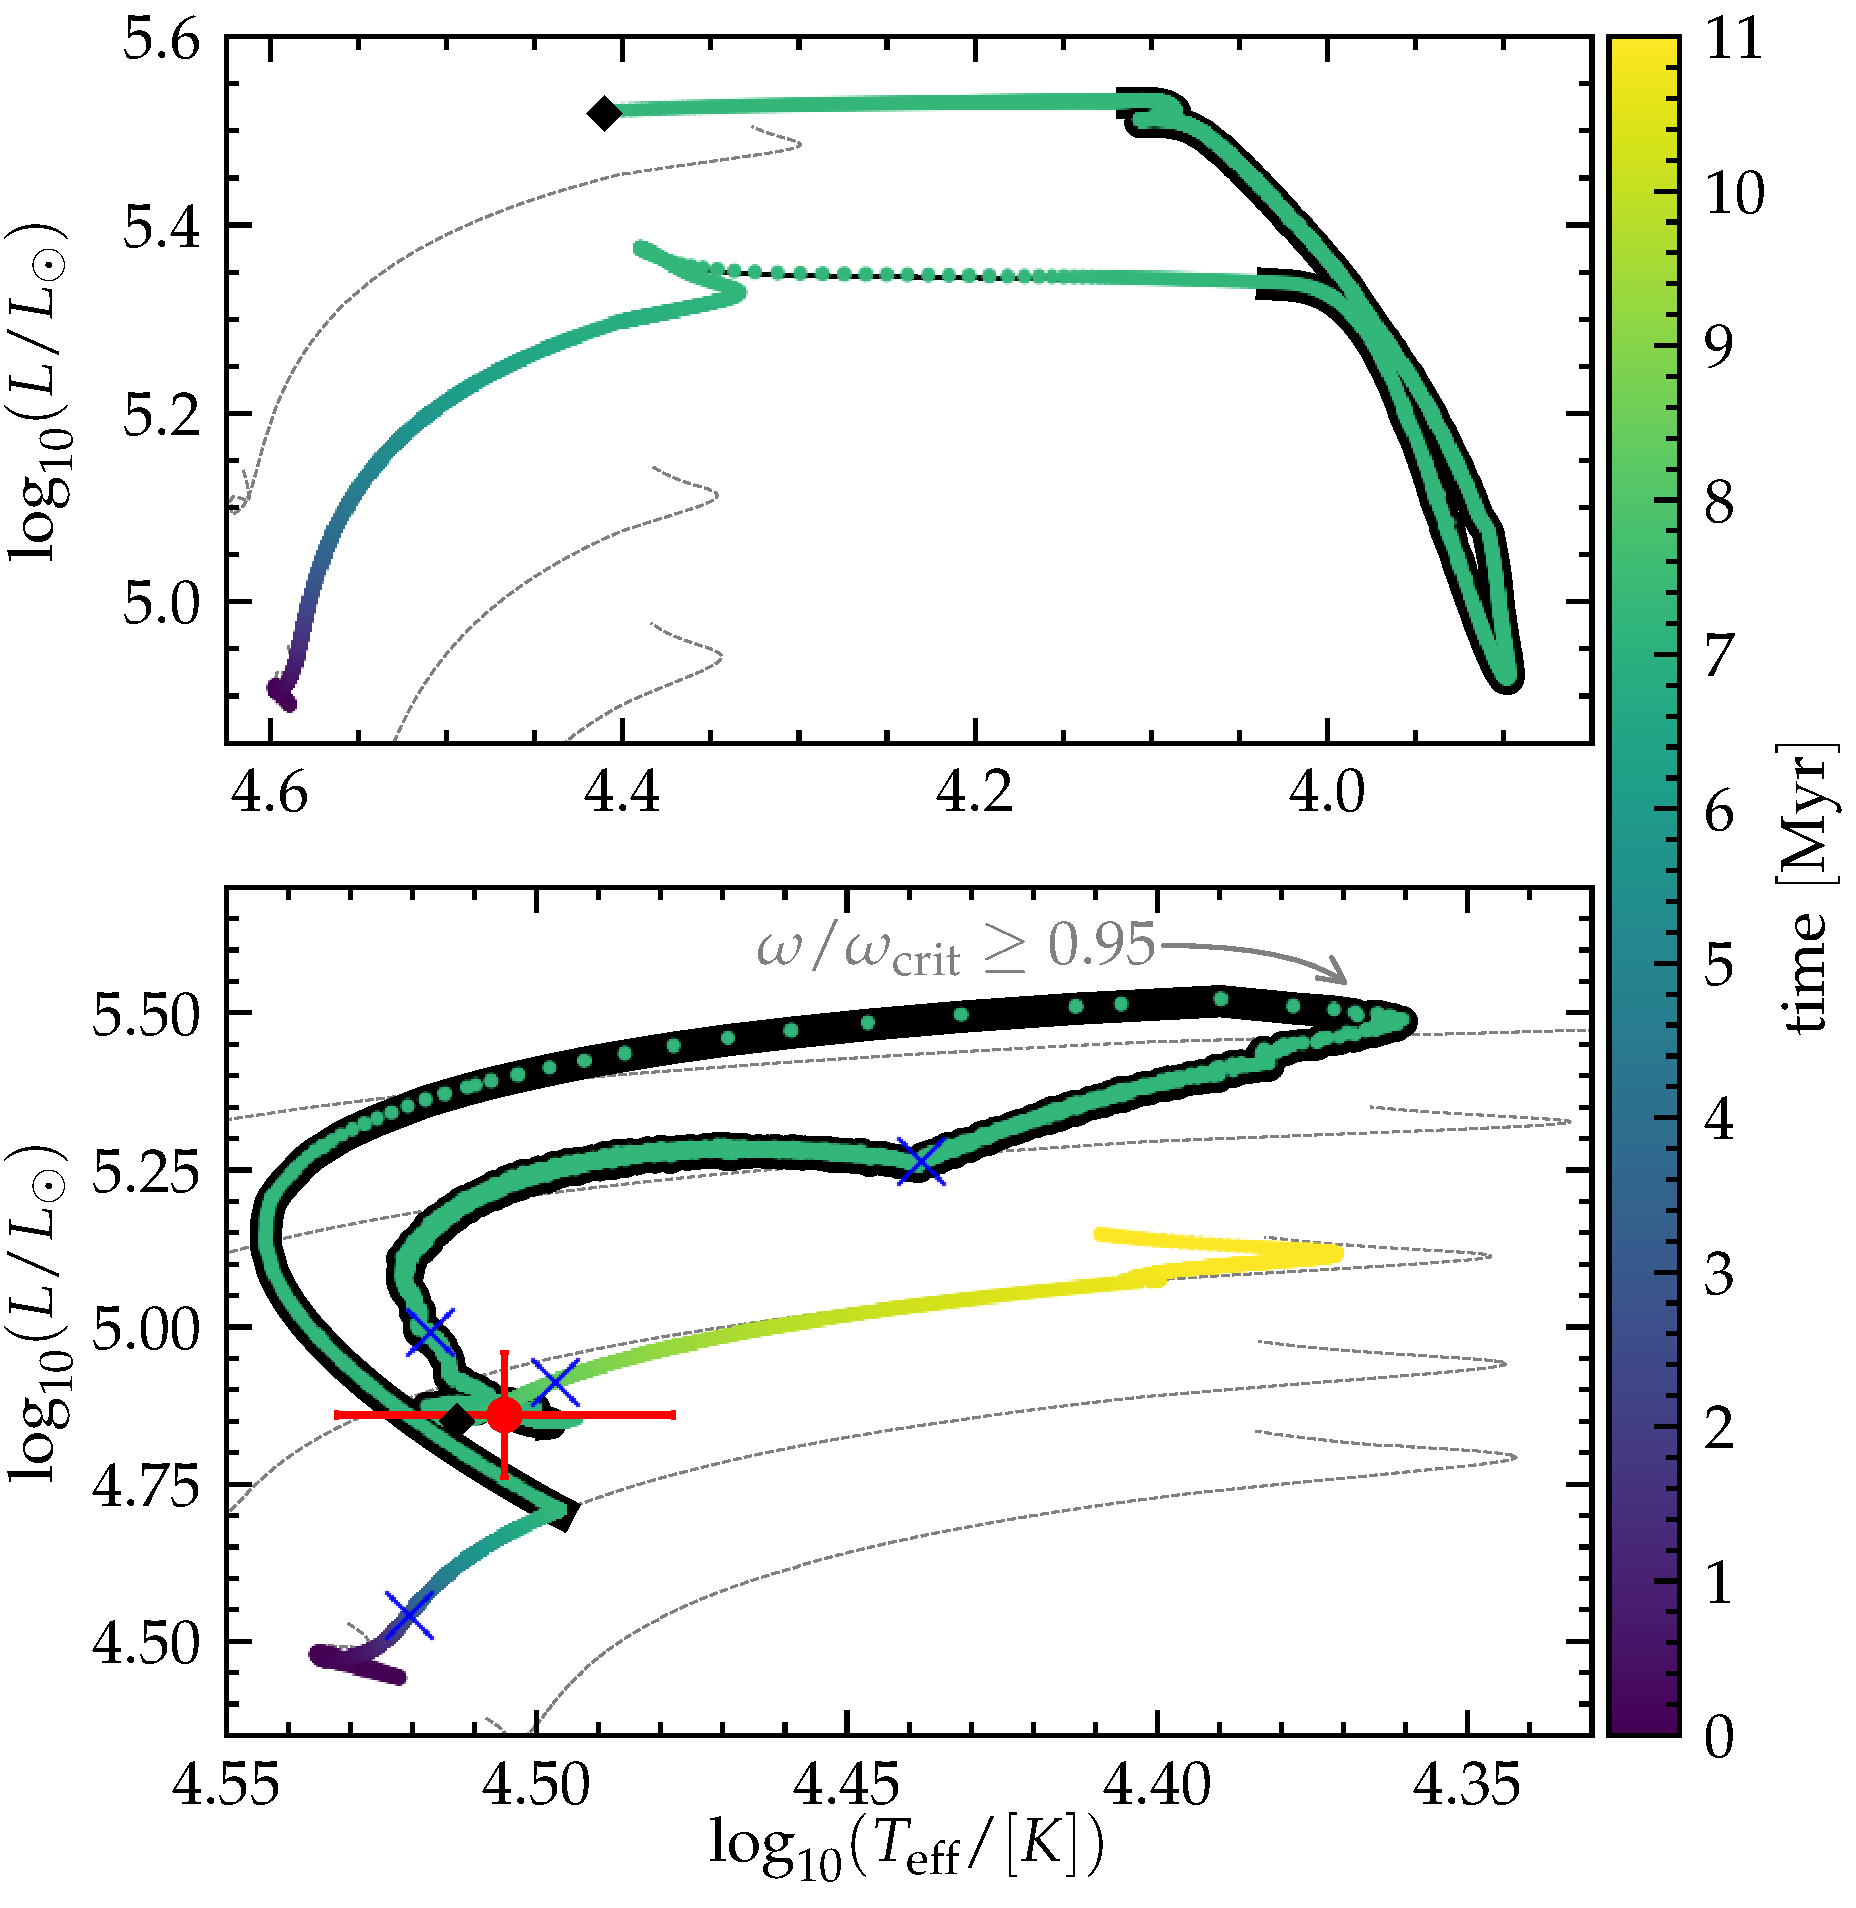
\includegraphics[width=0.5\textwidth]{HRD_both}
  \caption{HR diagram for the donor star (top) and accretor star (bottom) of
    the progenitor binary of \zoph. Each point is separated by 50
    years of evolution, and the part with a black outline corresponds
    to the RLOF phase. The colors represent the stellar age, the red
    data point shows the position of \zoph\ according to
    \citetalias{villamariz:05}, and the
    blue diamonds mark the end of the binary run. We
    continue the accretor evolution as a single star from there until
    core H depletion, hence the bottom panel shows a longer time. We
    emphasize the different scales on the two panels. The thin gray
    dashed line show the main sequence evolution of non-rotating
    single stars of 15, 17, 20, 25, and 30\,$M_\odot$ at $Z=0.01$ for
    comparison.}
  \label{fig:HRD_both}
\end{figure}

We describe here the evolution of a binary system where the accretor
star can broadly reproduces all the observed features of \zoph. We
assume initial masses $M_1=25\,M_\odot$, $M_2=17\,M_\odot$, and initial
period $P=100$\,days (corresponding to a separation
$a\simeq314\,R_\odot$) with a metallicity of $Z=0.01$.

\Figref{fig:HRD_both} shows the Hertzsprung-Russell (HR) diagrams of
both stars, the donor and accretor are shown separately on the top and
bottom panel, respectively (see \Figref{fig:sp_test} for an HR diagram of both stars on the same scale). After $\sim$$7.24$\,Myr, the donor star evolves off the main sequence and
$\sim8400$\,years later, at point A in \Figref{fig:HRD_both}, it overfills its Roche lobe. This results in a stable case B RLOF on a thermal timescale from point A to F (black outline of the curves). We refer to \cite{gotberg:17, klencki:20, laplace:21, blagorodnova:21} and references therein for a detailed description of the evolution of massive donor stars in binaries. Although our models are more massive, the qualitative behavior of the donor star is similar. Minor differences might arise because of mixing above and in the H-burning shell \citep[e.g.,][]{schootemeijer:19, klencki:21}, and its interplay with the mass transfer.

At the onset of RLOF (point A in \Figref{fig:HRD_both}), the accretor star is still on the main sequence with
$T_\mathrm{eff}\simeq10^{4.5}$\,K and its central mass fraction of hydrogen is $X(^1\mathrm{H})\simeq
0.42$. Because of accretion, it is pushed out of thermal equilibrium and quickly becomes over-luminous to radiate away the excess internal energy. The accretor reaches $L\simeq10^{5.5}\,L_\odot\gg
L_\mathrm{nuc}\simeq
10^{5.1}\,L_\odot$, with
$L_\mathrm{nuc}$ the total energy released per unit time by nuclear burning (integrated throughout the star).

The radius of the accretor increases dramatically from
$\sim7.5\,R_\odot$ to $\sim35\,R_\odot$, and only once the accretor
reaches critical rotation (roughly at point B in the bottom panel of
\Figref{fig:HRD_both}, roughly at the lowest $T_\mathrm{eff}$), the
star begins contracting and its $T_\mathrm{eff}$ increases. At
$T_\mathrm{eff}\simeq 10^{4.43}$\,K, slightly after point C, the
material transferred from the donor star becomes progressively more
He-rich and CNO-processed, changing the opacity in the outer-layers of
the accretor and causing a kink in its evolutionary track. This
indicates that the partially processed outer layers\footnote{These are
  left behind by the recession in mass coordinate of the core during
  the donor's main sequence.} of the donor's core are uncovered by
mass transfer.
Thus, late during the mass transfer material at high mean molecular
weight $\mu$ is put on top of the primordial envelope of the accretor,
modifying the morphology of the evolutionary track.

Because of the inverted $\mu$ gradient, thermohaline mixing starts in
the outer layers of the accreting star, and, together with rotational
mixing, it progressively dilutes the surface He and N mass fractions
and causes noisy features from point D to F on the HR diagram of the
accretor \citep[e.g.,][]{cantiello:07}. From D to E the donor star
briefly expands again: by point D the surface is He-rich, and partial
recombination of He drives a convective layer which is extremely thin
in mass ($\lesssim 10^{-4}\,M_\odot$) but can expand to significantly
large radii\footnote{With previous \texttt{MESA} releases, we found it
  challenging to compute our models beyond this phase: the large
  radius variation impacts significantly the mass transfer rate.}.

We emphasize that the (standard) algorithmic choices in
modeling mixing and rotation might impact the morphology of the
accretor's evolutionary track during RLOF. The entire duration of RLOF
from A to F is only about $10^4$\,years - of the order of the thermal timescale of
the donor star. Moreover, the accretor spends most of this time close
to the final, post-RLOF position (blue diamond in the bottom
panel). Therefore, the RLOF phase is unlikely to be observable to
probe directly the accuracy of our treatment of mixing. We expand on
the mixing processes inside the accretor in \Secref{sec:mixing}.

We evolve the binary system until the blue diamonds in
\Figref{fig:HRD_both}, which occurs well after the donor detaches from
the Roche Lobe. At this point, the accretor is a H-rich fast-rotating
star of
$\sim$$20.1\,M_\odot$. Available mass estimates for the presently single \zoph\ are highly uncertain, but most include
$20\,M_\odot$ (e.g., \citealt{hoogerwerf:01}, \citetalias{villamariz:05}, \citealt{neuhauser:20}). The accretor's post-RLOF orbital velocity is
$v_2\simeq52\,\kms$. In the subsequent evolution, wind mass loss from both stars will result in widening of the binary and slowing down the orbital motion of the accretor. We computed one binary until the end of the donor's He core burning, and at that point the accretor's orbital velocity has decreased to
$\sim$$40\,\kms$. Further decrease during the remaining evolution
is expected because of wind mass loss from both stars, likely dominated by the
(uncertain) mass-loss rate of the stripped donor star. Nevertheless,
the value we obtain is in broad agreement with estimates of the
observed runaway velocity of \zoph.

Accounting for both wind mass loss and the amount of mass transferred,
at the end of RLOF the donor becomes a He star of
$\sim$$9.4\,M_\odot$, likely to contract further. Depending on its wind mass-loss rate, the stripped donor's spectrum might show only absorption lines, only emission lines, or a mixture of both \citep[e.g.,][]{crowther:07, neugent:17, gotberg:18}. It's surface H mass fraction is $\lesssim
0.2$ and the layer still containing H will possibly be removed by further wind mass loss \citep[e.g.,][]{gotberg:17}.

After the donor detaches from its Roche lobe and contracts to a radius smaller than TAMS (blue diamonds in \Figref{fig:HRD_both}), we continue the evolution of the accretor as a single star with the same \texttt{MESA} setup until its TAMS. The main-sequence track on which the accretor settles post-RLOF has a higher luminosity compared to the original track because of the accretion of mass, and it has also a slightly steeper slope due to the close-to-critical rotation and the accretion of partially nuclearly processed material (He- and N-rich) material.

The red errorbars in the bottom panel of \Figref{fig:HRD_both} mark
the approximate position of \zoph\ based on the spectral analysis of
\citetalias{villamariz:05}. The color of the track in
\Figref{fig:HRD_both} indicate that our accreting star spends about
$\sim$2\,Myr within the represented errorbars after the end of
RLOF. Assuming the kinematic age of $1.78\pm0.21$
\citep{neuhauser:20}, together with the remaining lifetime of the
donor of $\sim$0.5\,Myr, our model approximately produces the correct
timescale for the binary SN scenario.



\begin{figure}[htbp]
  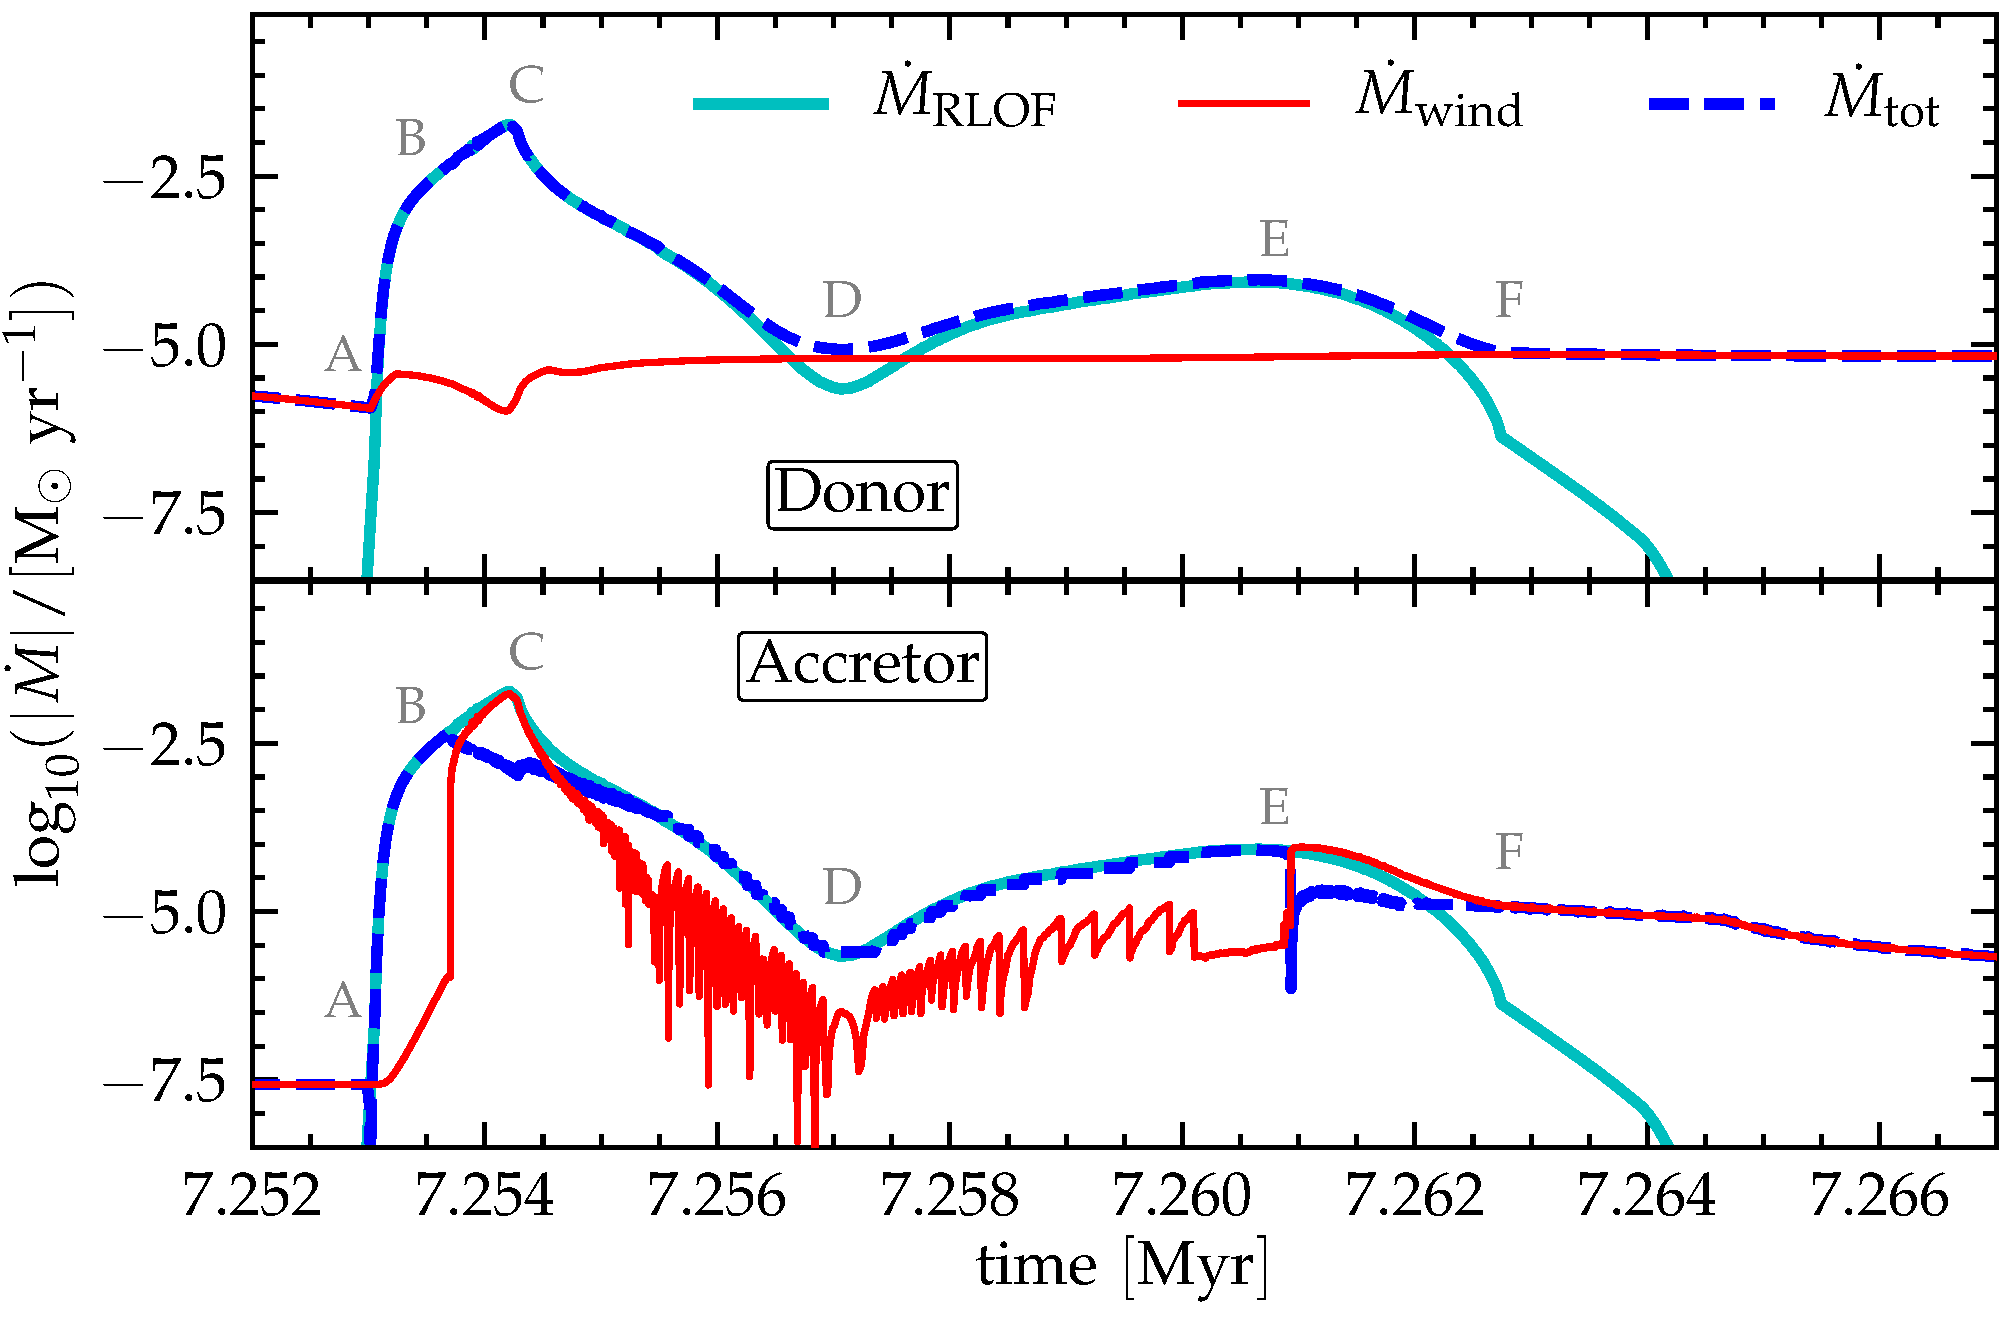
\includegraphics[width=0.47\textwidth]{MT}
  \caption{The top panel shows the total mass of each star as a
    function of time during RLOF. The middle and bottom panel show a break down of
    the mass transfer rates for the donor and accretor star,
    respectively. In these, the cyan solid lines show the mass transfer rate
    due to RLOF, the red lines show the (mechanically
    enhanced) wind mass loss rates, and dashed blue lines show the actual
    change in the mass of the stars (due to the combination of wind,
    and accretion). During RLOF the accretor reaches
    critical rotation, which leads to oscillations in the
    rotationally-enhahnced wind mass loss.}
  \label{fig:MT}
\end{figure}

\Figref{fig:MT} shows the mass evolution (top panel) and the rate of
mass change (middle and bottom panel) for each star during
RLOF. The middle panel focuses on the donor star which loses mass via RLOF
(cyan line) and winds (thin red line). The dashed blue lines
show their combination resulting in the actual rate of mass change of
the stars. The bottom panel shows instead the accreting star, which
grows in mass because of the mass transfer. At peak (point C), the mass transfer
rates reaches values above
$10^{-2}\,M_\odot\ \mathrm{yr^{-1}}$ and taps into the optically
thick matter of the donor (i.e., the donor Roche radius becomes
smaller than its photosphere $R_\mathrm{RL,1}<R_1$).

Initially, between point A and B, the mass transfer rate equals the mass accretion rate
(bottom panel of \Figref{fig:MT}), that is initially the accretion is
(by construction) fully conservative. The bulk of the mass is accreted
during this initial phase which lasts about $\sim{}2\times10^3$\,years. As the mass and surface rotation
rate of the accretor increase, the assumed rotational-enhancement of
the wind progressively increases the mass-loss rate by $\sim$5 orders
of magnitude. The mechanically-enhanced wind
controls the accretion efficiency, and at
$\sim$$7.254$\,Myr (from B to C, where the red solid line and the cyan line overlap) the mass transfer becomes briefly non-conservative: the majority of the mass transferred during this phase is ejected, we assume as a fast wind from the vicinity of the accretor. Consequently, the accretor slightly spins down and starts contracting (cf.~\Figref{fig:HRD_both}).
In the remaining evolution from C to F, the interplay between the wind mass loss rate, the spin-up due to accretion and the spin-down due to inward transport of angular momentum (see \Secref{sec:rot}) trigger oscillations in the wind mass loss rate. Nevertherless, for most of the evolution, accretion, albeit not-fully conservative, still occurs. This allows for CNO-processed material from the donor to reach the surface of the accretor during late stages of mass transfer.

The minimum of the mass transfer rate in point D corresponds to a brief phase of contraction (see also \Figref{fig:HRD_both}). However, from D-E, the donor star briefly expands again
($T_\mathrm{eff}\simeq10^{4.1}$\,K, $L\simeq10^{5.5}\,L_\odot$). This
is due to the partial recombination of the now He-rich outer layers,
which causes a transient surface convection layer. This causes a
radial expansion of the outer convective layers and an increase in the
mass-transfer rate, despite at this point the donor is less massive
than the accretor and the binary is widening.  During this phase, the
mass transfer becomes non-conservative again (in the bottom
panel the wind and the mass accretion rate nearly cancel each other again
at $\sim7.261$\,Myr), until the donor completely detaches from its Roche lobe at point F.

\subsection{Mixing and composition}
\label{sec:mixing}

\begin{figure}[htbp]
  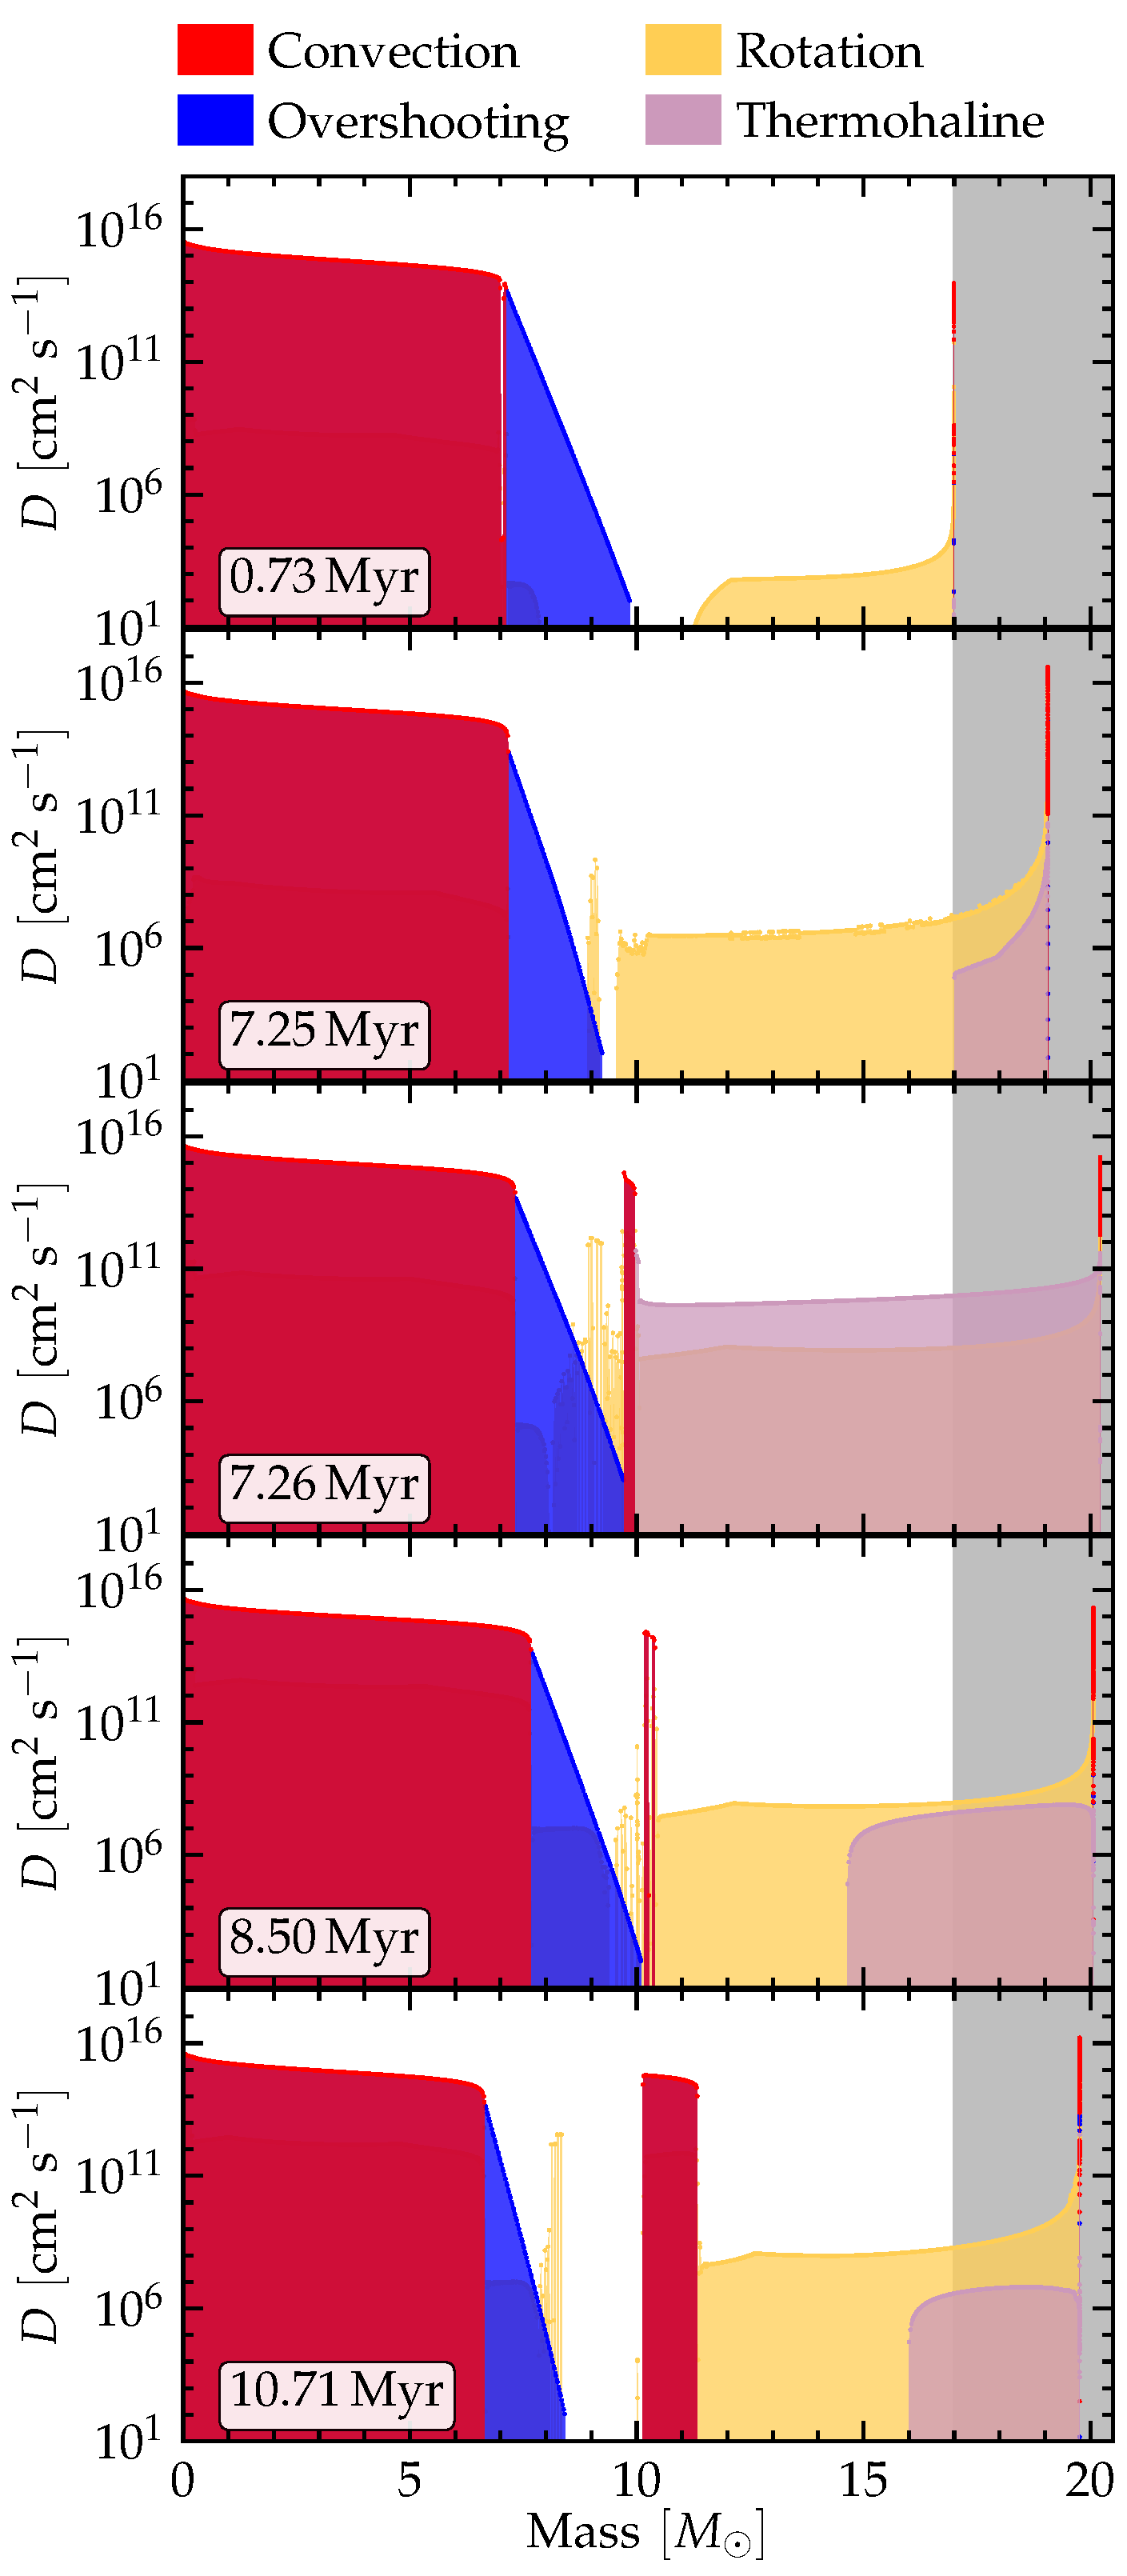
\includegraphics[width=0.47\textwidth]{D_mix_vertical}
  \caption{Mixing diffusion coefficients in the accretor star. The
    gray area on the left highlights accreted material. From
    top to bottom, each panel shows a profile during the main sequence
    (before point A in \Figref{fig:HRD_both}),
    early during RLOF (close to point C), mid-RLOF (close to
    point D), late during RLOF (between point D and E), and after RLOF
    (point G). A movie of the entire evolution is available at \todo{zenodo}.}
  \label{fig:D_mix}
\end{figure}

\texttt{MESA} treats mixing in the diffusion approximation
\citep{paxton:11}. To illustrate the dominant processes throughout the
accretor's evolution, we show in \Figref{fig:D_mix} the diffusion
coefficients for various mixing processes as a function of mass
coordinate at selected times. Specifically, we show from top to
bottom:
\begin{itemize}
\item main sequence before RLOF (i.e., before point A in
  \Figref{fig:HRD_both} and \Figref{fig:MT});
\item beginning of RLOF (between point A and B);
\item late during RLOF (between point C and D);
\item predicted present-day structure of \zoph\ (post-RLOF within the
  red error-bar on \Figref{fig:HRD_both});
\item close to TAMS (point G in \Figref{fig:HRD_both}).
\end{itemize}
In each panel, the gray shaded areas highlight mass accreted during RLOF.
The colors in \Figref{fig:D_mix} show convection (red), overshooting
(blue), rotational mixing (yellow), and thermohaline mixing
(pink). Rotational mixing includes all the rotational instabilities
that we consider -- meridional currents, secular and dynamical shear instabilities,
and GSF instability, but throughout the evolution
it strongly dominated by Eddington-Sweet meridional circulations,
except at the interface between core-envelope (i.e., at the outer edge
of the overshooting region), where the post-RLOF contraction and
spin-up of the core (see \Secref{sec:rot}) can lead to significant
dynamical shear (and GSF mixing to a lesser extent).
For clarity, we do not show semiconvection
which is never the dominant mixing process in our model.

The top panel shows the typical structure of a main sequence massive star:
the convective core initially reaching
$\sim$$7\,M_\odot$ with the overshooting extension to $\sim$$9\,M_\odot$. The
slow rotation imparted by the assumed initial tidal synchronization
causes a meridional circulation in the envelope. Meridional
circulations are also present in the core throughout the evolution,
but with a diffusivity more than nine orders of magnitude lower than
core convection. A small sub-surface
convective zone is also appreciable at the very surface (see, e.g., \citealt{cantiello:21}).

In the second panel from the top, the star has already accreted
$\sim$$2\,M_\odot$ (extending in the gray region), and its surface is already spun up to $\sim
330\,\kms$. Thermohaline mixing has started in the newly accreted layers, but it is subdominant compared to rotational mixing due to meridional circulations in the envelope.  Angular momentum transport (by the Spruit-Tayler dynamo) has already imparted some rotation to the inner layers of the envelope. This leads to the disconnected spike in rotational mixing at the outer edge of the core, dominated by dynamical shears.  We note that between the top panel and the onset of RLOF, the convective core receeds in mass coordinate, but, by the time shown in the second panel, the accretion of mass has caused the core to grow back to its initial size.

In the third panel, the star has already accreted all the mass that it will, including CNO-enriched layers from the donor's interior. Thermohaline mixing takes over the dominant role in the envelope (although meridional circulations persist behind it). The increase in core-mass causing the rejuvenation effect is still going on, and the mixing at the core-envelope boundary is partially still due to dynamical shear, but an off center convective region also appears. Because we adopt an exponentially decreasing overshooting, the diffusion coefficient at the outer edge of the overshooting region is small, and the mixing between the core and the off-center convective region is weak. We do not include over/undershooting for off-center convective layers, which could increase the coupling between these layers. By the fourth panel, roughly corresponding to \zoph's structure today, thermohaline mixing is progressively shutting down, but some residual mixing at the core edge still remains.


    % this table was automatically generated using the table.ipynb in the repository associated to this manuscript
    \begin{table*}[hbpt]
    \centering
    \begin{tabular}{c|c|c|c|c|c|c|c|c}
    \hline\hline
    $M \ [M_\odot]$ & $R\ [R_\odot]$ & $\log_{10}(\omega / [\mathrm{s^{-1}}])$ & $v_\mathrm{rot} \ [\kms] $ & $X(^{1}\mathrm{H})$ & $X(^{4}\mathrm{He})$ & $X(^{12}\mathrm{C})$ & $X(^{14}\mathrm{N})$ & $X(^{16}\mathrm{O})$ \\
    \hline
    20.1 & 9.6 & -4.263 & 366.1 & 0.678010 & 0.312093 & 0.001344 & 0.001340 & 0.004148 \\
    \hline
    \end{tabular}
    \caption{Properties of the accretors shortly after the end of RLOF
    (last thin blue cross in \Figref{fig:HRD_both})}
    \label{tab:surf_prop}
    \end{table*}
    


Finally, the last panel shows that as the post-RLOF evolution
proceeds, the convection at the outer-edge of the core advances
further and remains as a long-lived
$\sim$$1\,M_\odot$ wide region above the core, but disconnected from it. This is a consequence of core growth because of accretion, and can affect the density profile at the base of the envelope (see
also \Figref{fig:rho} for its effect on the density profile).

The core growth caused by the accretion of mass, the
consequent ingestion in the burning region of fresh H-rich material, and the
resulting rejuvenation of the accretor are strongly dependent on the presence of
convective boundary mixing. In our model this is initially provided by
overshooting and to a lesser extent dynamical shear (between the top
and second panel), at later times, the development of a convective
layer above the overshooting region dominates this mixing.

Instead, in the envelope, Eddington-Sweet circulations first dominate,
then (roughly from the kink after point C in \Figref{fig:HRD_both}
until the end of RLOF) thermohaline mixing takes over. The combination
of these two processes mixes inward material CNO processed in the
donor star and accreted from the surface, and outward CNO processed
material from the core of the accretor.

\Tabref{tab:surf_prop} summarizes the surface properties of the
accretor star at the time shown in the fourth panel of
\Figref{fig:D_mix}, roughly corresponding to \zoph\ today. Both the
mass and radius agree reasonably well with the estimates from
\citetalias{villamariz:05} and previous studies, that is~$20\,M_\odot$
and $8.3\pm1.5\,R_\odot$, respectively. Our radius of $9.8\,R_\odot$
is larger by $\sim0.6\,R_\odot$ than the equatorial radius recently
measured by \cite{gordon:18}, and our model has a
$T_\mathrm{eff}\simeq31\,300$\,K, on the lower end of the range considered by
\citetalias{villamariz:05}. On the other hand, the age of
$8.5$\,Myr is maybe slightly lower than \zoph's
kinematic age plus the entire donor's lifetime. The surface rotational velocity in excess
of $350\,\kms$ is also in the correct ballpark albeit possibly on the
low end. We discuss further rotation and angular momentum transport in
\Secref{sec:rot}.

We report the surface H mass fraction\footnote{We obtain the mass
  fractions of individual elements inverting the definition
  $\varepsilon(X)=12+\log_{10}(N_X/N_H)$, where $N_X$ and $N_H$ are
  the number fractions of species $X$ and H, respectively
  \citep[e.g.,][]{lodders:19}.}, lower than primordial because of the
accretion of nuclearly processed material, and the surface mass
fraction of the most prominent species $^4\mathrm{He}$,
$^{12}\mathrm{C}$, $^{14}\mathrm{N}$, $^{16}\mathrm{O}$.  Assuming our
surface H mass fraction $X(^1\mathrm{H})$, the corresponding mass
fractions of $^4\mathrm{He}$, $^{12}\mathrm{C}$, $^{14}\mathrm{N}$,
$^{16}\mathrm{O}$ obtained by \citetalias{villamariz:05} are
$0.34^{+0.14}_{-0.05}$, $0.0006\pm0.0004$, $0.002\pm0.001$, and
$0.005\pm0.004$.

By the accretor's TAMS, rotational mixing (in the
form of Eddington-Sweet circulations) and thermohaline mixing nearly
homogenize the composition of the envelope of our accretor's
model. The surface mass fractions we obtain are sensitive to the
interplay between several poorly understood processes treated in one
dimension: mass accretion efficiency, rotationally enhanced wind mass
loss, thermohaline, and inward rotational mixing. These also impact
the composition of the envelope, and thus its radius and
$T_\mathrm{eff}$. Therefore, although not perfect, we consider the
match with the mass fractions reported by \citetalias{villamariz:05}
surprisingly satisfactory.

\begin{figure*}[htbp]
  \centering
  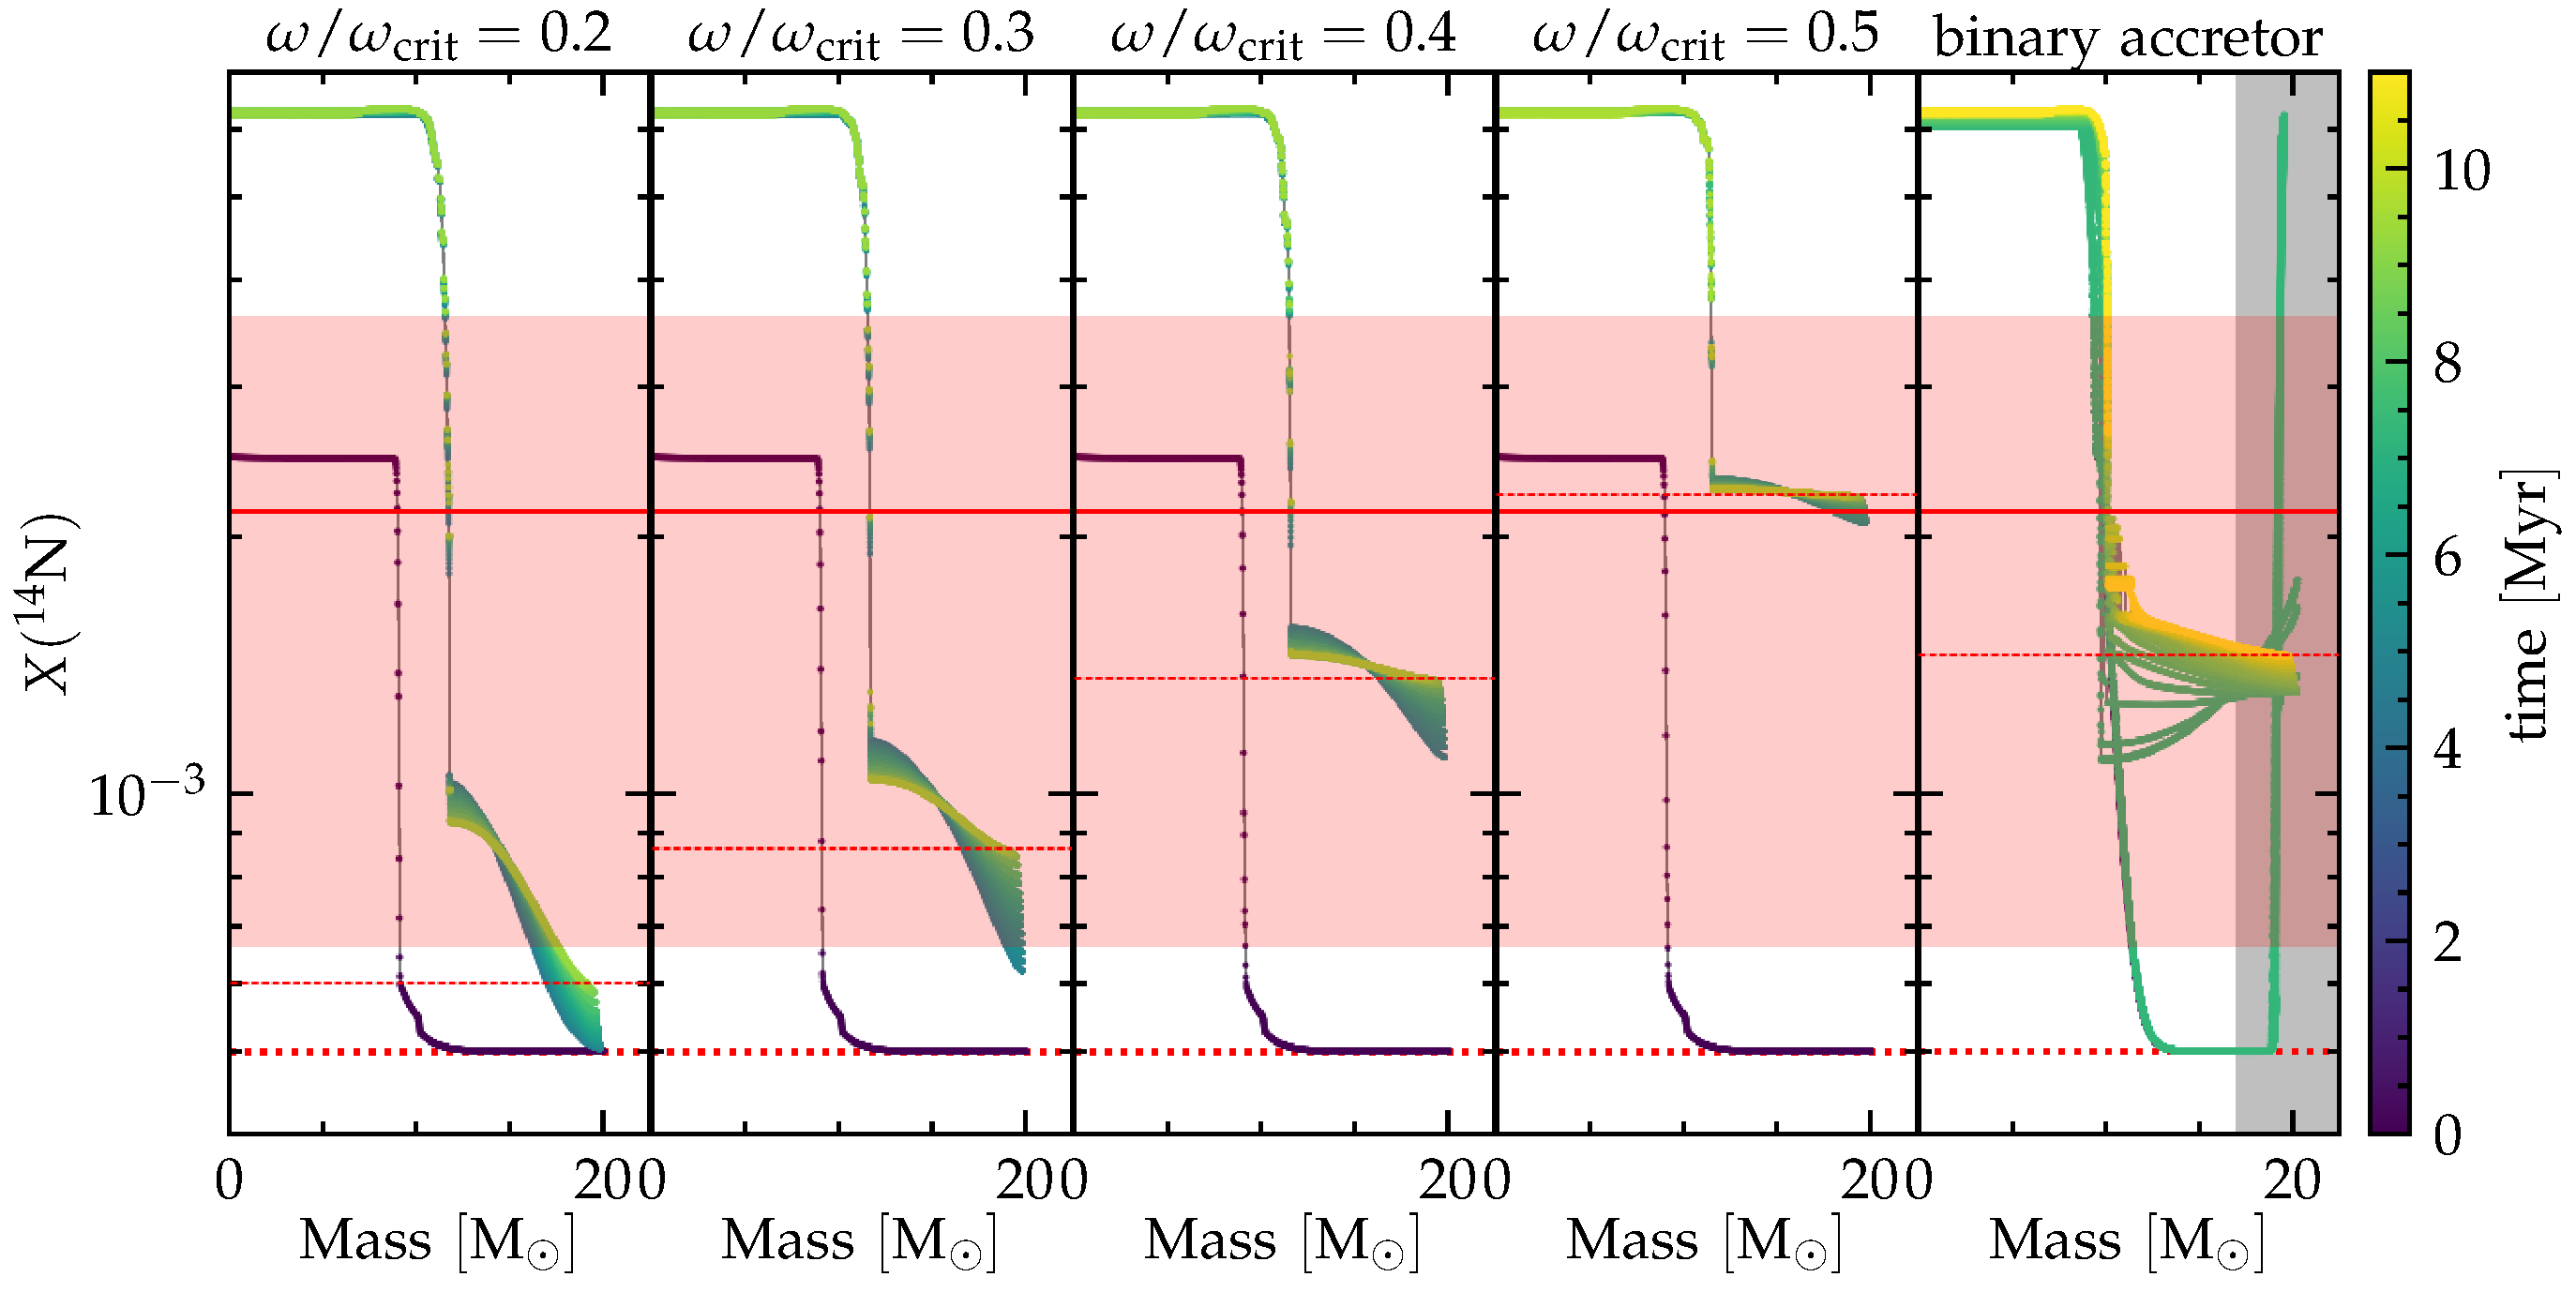
\includegraphics[width=\textwidth]{n14_struct_complete_zeta_ab}
  \caption{$^{14}\mathrm{N}$ mass fraction as a function of mass
    coordinate for $20\,M_\odot$ single star models with increasing
    $\omega/\omega_\mathrm{crit}$ at birth (first four panels), and
    for the accretor of our fiducial binary (last panel). In each
    panel, the darkest flat line marks the primordial value for
    $Z=0.01$, the dashed red line marks the surface value at TAMS. The
    colors of each profile go from dark to light at TAMS, and selected
    profiles along the main sequence are shown.  In
    the last panel, the gray area highlights mass accreted during
    RLOF, and the black dashed line corresponds to the internal
    structure at the black
    diamond in \Figref{fig:HRD_both}. The solid red line and
    the shaded red region correspond to the mass fraction of
    $^{14}\mathrm{N}$ estimated by \citetalias{villamariz:05} assuming
    the surface mass fraction of H from \Tabref{tab:surf_prop}. The
    abundance of $^{14}\mathrm{N}$ alone is not strongly
    constraining. \Figref{fig:composition_huge} shows a similar plot
    containing also $^{12}\mathrm{C}$ and $^{16}\mathrm{O}$.}
  \label{fig:n14}
\end{figure*}

\subsubsection{Comparison to single fast-rotating stars}
\label{sec:mix_comparison_single}

We now compare the mixing processes
in our accretor and in single rotating massive star models. The first
four panels of \Figref{fig:n14} show the mass fraction of $^{14}\mathrm{N}$
as a function of mass coordinate along the evolution of four
$20\,M_\odot$ stars initialized with
$\omega/\omega_\mathrm{crit}=0.2,0.3,0.4,0.5$. Except for the initial rotation rate and
being single, these stars have the same \texttt{MESA}
setup as our binary model. The last panel of \Figref{fig:n14} shows
our accretor model. The thin
dashed lines mark the surface mass
fraction of $^{14}\mathrm{N}$ at TAMS, while the primordial value for
the adopted $Z=0.01$ is shown by the ZAMS profiles (dark purple).

The colored tracks show selected profiles throughout the main
sequence, with lighter colors corresponding to more evolved stars. The
accretor model (rightmost panel) starts as a 17$\,M_\odot$ and is
rejuvenated by binary interactions, reaching TAMS at
11.2\,Myr. For comparison, the lifetime of a non-rotating single star
of 17\,$M_\odot$ is $\sim$11.1\,Myr, while the initially 20\,$M_\odot$
rotating models have a main-sequence lifetime of $\sim$9.2-9.6\,Myr (longer
for higher initial rotation rates), hence their TAMS profile does not
have as light a color in \Figref{fig:n14}.

The first four panels of \Figref{fig:n14} show the typical rotational
mixing profiles: $^{14}\mathrm{N}$ rapidly rises in the core because
of the CNO burning, and it is then mixed outwards (as indicated by the
arrows in the top left corner of each panel). At any time
the $^{14}\mathrm{N}$ profile is monotonically decreasing in mass
coordinate, and the higher the initial rotation, the higher the
surface $^{14}\mathrm{N}$ mass fraction reached at TAMS.

Conversely, the $^{14}\mathrm{N}$ mass fraction profile of the
accretor is \emph{not} monotonic throughout the evolution.  The
profile is shaped by two main processes: (i) accretion of
CNO-processed material from the donor star mixed inwards by meridional
circulations and thermohaline mixing (as indicated by the top right arrow
in the last panel), (ii) outward mixing of the
CNO-processed material from the accretor's core caused by rotational
mixing -- as in the single stars -- and rejuvenation.

Initially, the tidally synchronized accretor star
rotates too slowly ($\lesssim 3\,\kms$) for significant outward rotational mixing out of
the core, and until the onset of RLOF (roughly at 7.25\,Myr) no appreciable variation of the
envelope $^{14}\mathrm{N}$ mass fraction occurs. During late RLOF after the
``kink'' feature bewteen C and D in \Figref{fig:HRD_both}, N-enriched material from the
donor's core piles onto the accretor's surface -- inside the gray
area. The close-to-critical
rotation (through Eddington-Sweet circulations) and the inversion in the mean molecular
weight $\mu$ (through thermohaline mixing) drive inward mixing of
the N-rich material and dilute it in the envelope (see also \Figref{fig:D_mix}).

Simultaneously, the mere growth in mass causes the steepening of the
core-temperature gradient and increase in the convective core mass
\citep[rejuvenation, e.g.,][]{schneider:16}, driving some outward
convective mixing of N-rich material. This also causes the formation
of an off-center convective region (cf.~\Figref{fig:D_mix}) which
persists until TAMS. Because convection turnover timescale is much
shorter than evolutionary timescales, convection homogenizes the
composition of this region and produces ``steps'' at
the outer edge of the core (slightly outside mass coordinate
10\,$M_\odot$).

In \Figref{fig:n14}, the solid red line and red shaded area across all panels show the
$^{14}\mathrm{N}$ from \citetalias{villamariz:05} (assuming the
surface H mass fraction from our model listed in
\Tabref{tab:surf_prop}). The mass fraction of $^{14}\mathrm{N}$
alone is not sufficient to distinguish between these models, and already
a moderate $\omega/\omega_\mathrm{crit}\geq0.3$ is sufficient for
models to reach the lower-limit of the error bar.


\subsection{Angular momentum transport and surface rotation}
\label{sec:rot}

One of the main distinguishing features of \zoph\ is its extremely
high surface rotation rate.
The black line in the top panel of \Figref{fig:surf_rot} shows the
evolution of the surface equatorial rotational velocity
$v_\mathrm{eq}$ for our accretor model, not including any projection
effect. More precisely, $v_\mathrm{eq}$ is a mass-weighted average of
the rotational velocity of layers with opacity
$\tau\leq 100$. The dark horizontal red band corresponds to the
$v\sin(i)=432\pm16\,\kms$ measured by \cite{zehe:18}, and the lighter
band shows a range of 5 times their error bar, which roughly encloses
the majority of the estimated $v\sin(i)$ for \zoph\ in the literature
down to $\sim$$350\,\kms$.  For comparison, the colored solid lines show also
$v_\mathrm{eq}$ for single rotating
$20\,M_\odot$ stars of varying initial
$\omega/\omega_\mathrm{crit}$.  The bottom panel of \Figref{fig:surf_rot} shows instead the ratio
of the surface rotational frequency $\omega_\mathrm{surf}$ to $\omega_\mathrm{crit}$.

\begin{figure}[tbp]
  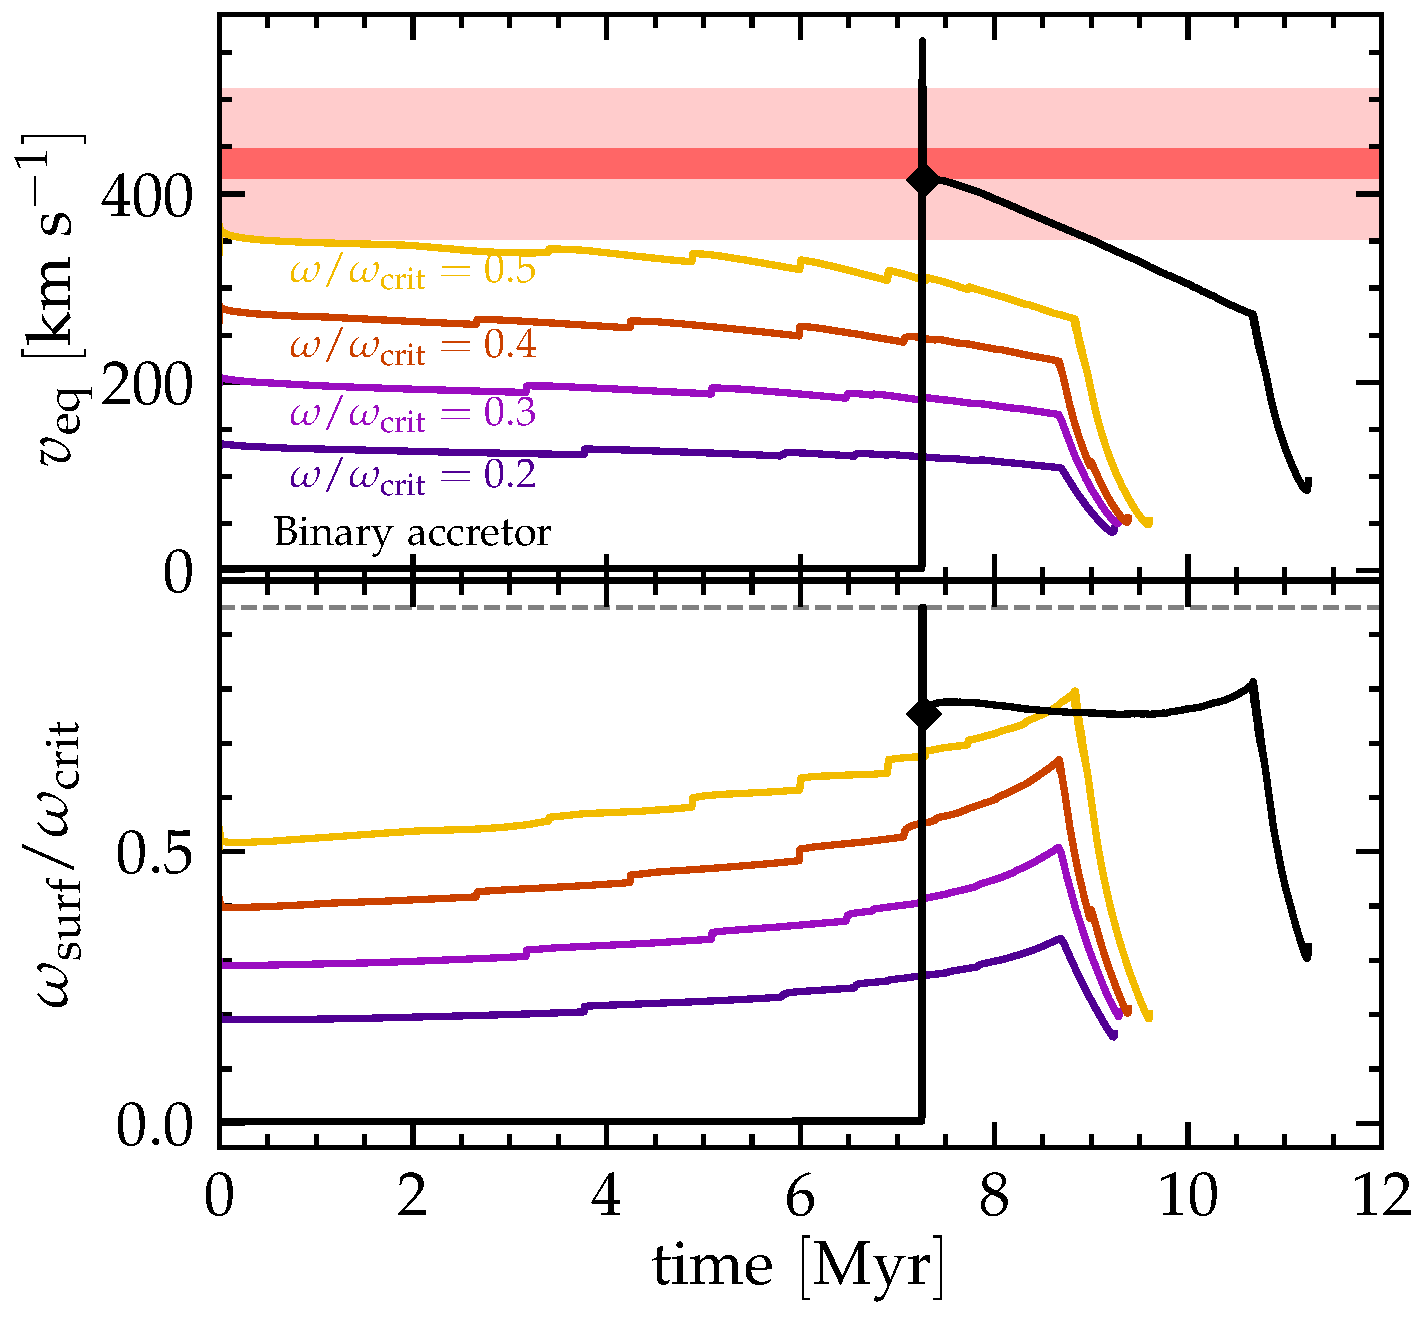
\includegraphics[width=0.5\textwidth]{zeta_rot}
  \caption{Equatorial surface rotational velocity (top panel) and
    $\omega/\omega_\mathrm{crit}$ (bottom panel) for the accretor model (black) and single rotating
    $20\,M_\odot$ stars (colored lines). At
    $\sim$7.25\,Myr the mass transfer quickly spins up the accretor to critical rotation: the dashed horizontal line in the bottom panel shows the upper-limit we impose. By the time the donor detaches from the RLOF the accretor is still spinning at
    $\sim$$400\,\kms$. From this point (blue diamonds) onwards, we
    continue the evolution as a single star, and the accretor spins
    down because of wind mass loss.  Note however that we use the wind
    mass-loss rate from \cite{vink:01}, which might be $\sim$2 orders
    of magnitude too high for \zoph\ \citep{marcolino:09}.}
  \label{fig:surf_rot}
\end{figure}



The initial binary is wide enough that assuming tidal synchronization
at ZAMS implies a very low rotation. At 7.25\,Myr, RLOF rapidly spins
up the accretor to critical rotation, up to
$v_\mathrm{crit}\simeq520\,\kms$ (this value is also mass-averaged
over the region with $\tau<100$). This corresponds to
$\omega/\omega_\mathrm{crit}\simeq 0.95$ (dashed horizontal line in
the bottom panel of \Figref{fig:surf_rot}), which is the upper-limit
we impose in our models.

The star remains fast rotating throughout the mass transfer phase,
which ends at the blue diamond in \Figref{fig:surf_rot}. In the
remaining evolution, the star spins down progressively through wind
mass loss, and within $\sim$2\,Myr its averaged surface rotational
velocity drops below
$\sim$$350\,\kms$. Both the single star models and our accretor (after being spun up) evolve to higher
$\omega/\omega_\mathrm{crit}$ because of the increase in stellar radii and corresponding decrease in
$\omega_\mathrm{crit}$ \citep[e.g.,][]{langer:98, zhao:20}. However, our accretor remains at a higher
$\omega_\mathrm{surf}/\omega_\mathrm{crit}$ for a significantly longer time: the chance of observing a single rotating star at very high
$\omega_\mathrm{surf}/\omega_\mathrm{crit}$ is lower than for an accretor from a massive binary system. Close to the end of the main sequence, the increase in wind mass loss rate and internal transport of angular momentum strengthen the surface spin-down. This effect is also seen in the late main-sequence evolution of single stars rotating rapidly from ZAMS.

\Figref{fig:surf_rot} shows that our model can retain a significant surface rotation for a time comparable to the kinematic age of the star, which is shorter than the remaining main-sequence lifetime. Since the spin up of the accretor happens roughly half-way through its main-sequence, the star is much faster rotating than single stars of the same (post-RLOF) mass initialized as fast rotators at ZAMS. Although \Figref{fig:surf_rot} does not account for the projection angle, \cite{zehe:18} argued for
$i\geq56$\,degrees, corresponding to an upward shift of the red band in \Figref{fig:surf_rot} of $\lesssim
20\%$. This has the same impact on our accretor model and on single star models of \zoph.

We emphasize that our model is computed using the \cite{vink:00,
  vink:01} wind mass-loss rate with full efficiency throughout its
evolution. This is two orders of magnitude higher than the wind mass
loss rate reported by \cite{marcolino:09} (weak wind problem,
however, see also \citealt{lucy:12, lagae:21}). While this may impact
the evolution of the binary even before RLOF, it presumably increases the
spin-down rate of our model compared to the observations. We expect
that an accreting star modeled with lower wind-mass loss rate
post-RLOF would retain an even higher surface rotation for longer (see
also \Secref{sec:single_star_uncertainties}).


\subsubsection{Comparison to single fast-rotating stars}

\begin{figure*}[tbp]
  \centering
  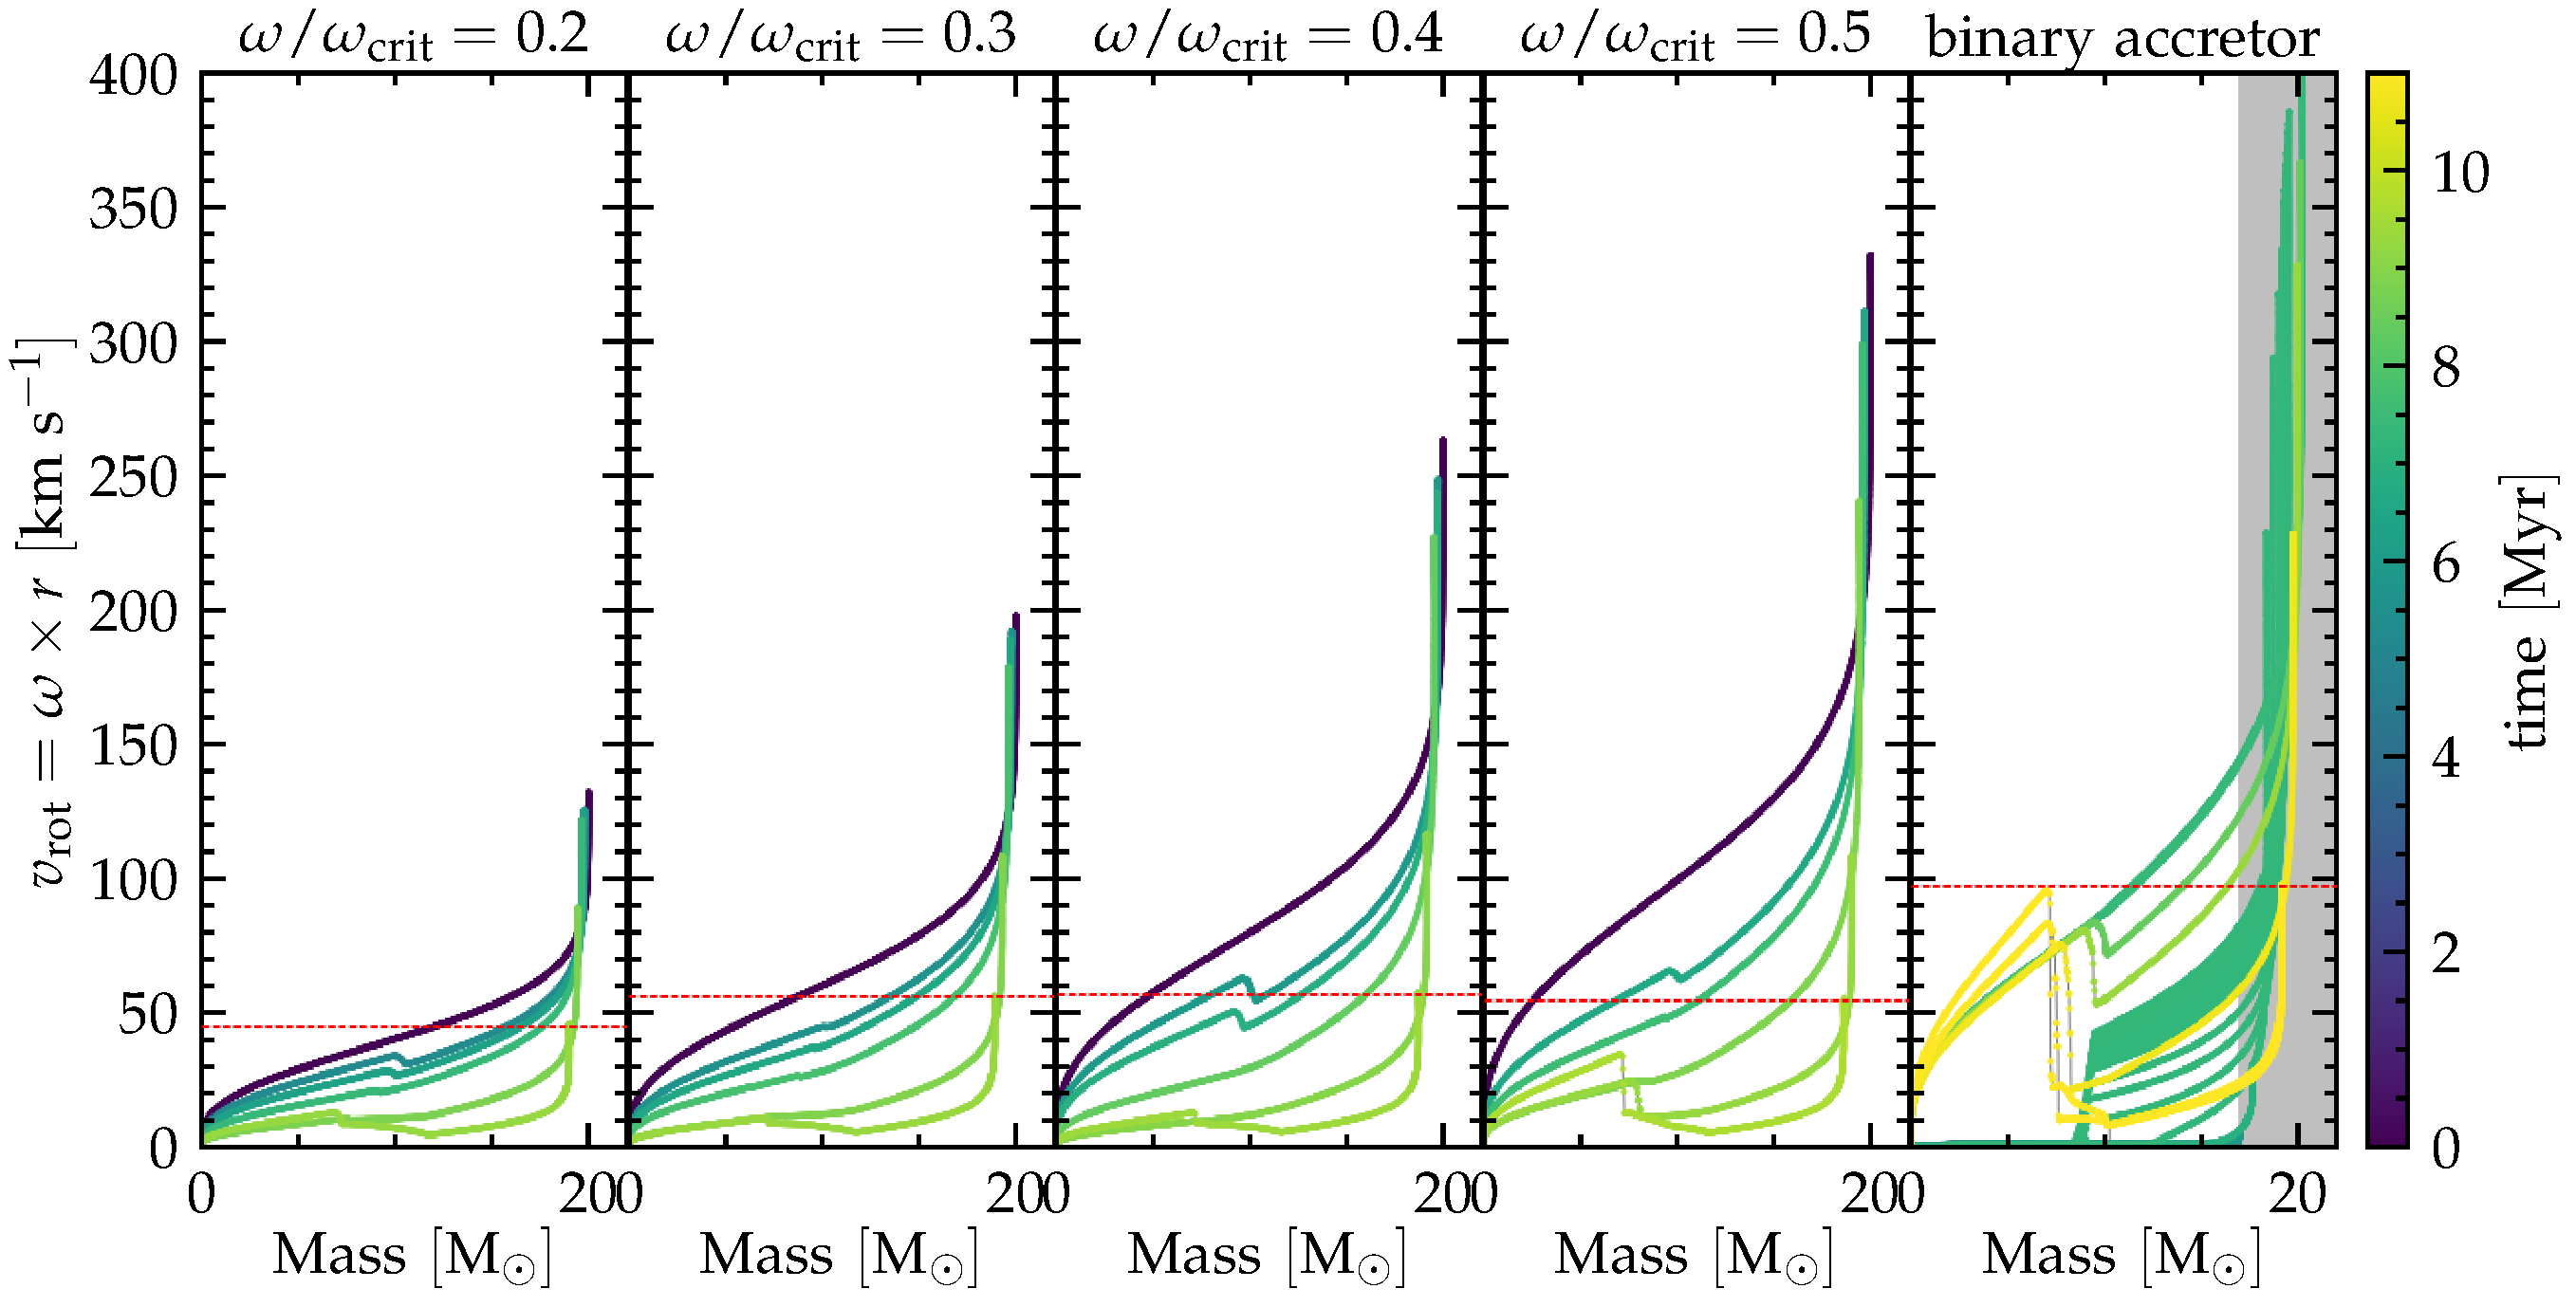
\includegraphics[width=\textwidth]{zeta_Rotational_struct}
  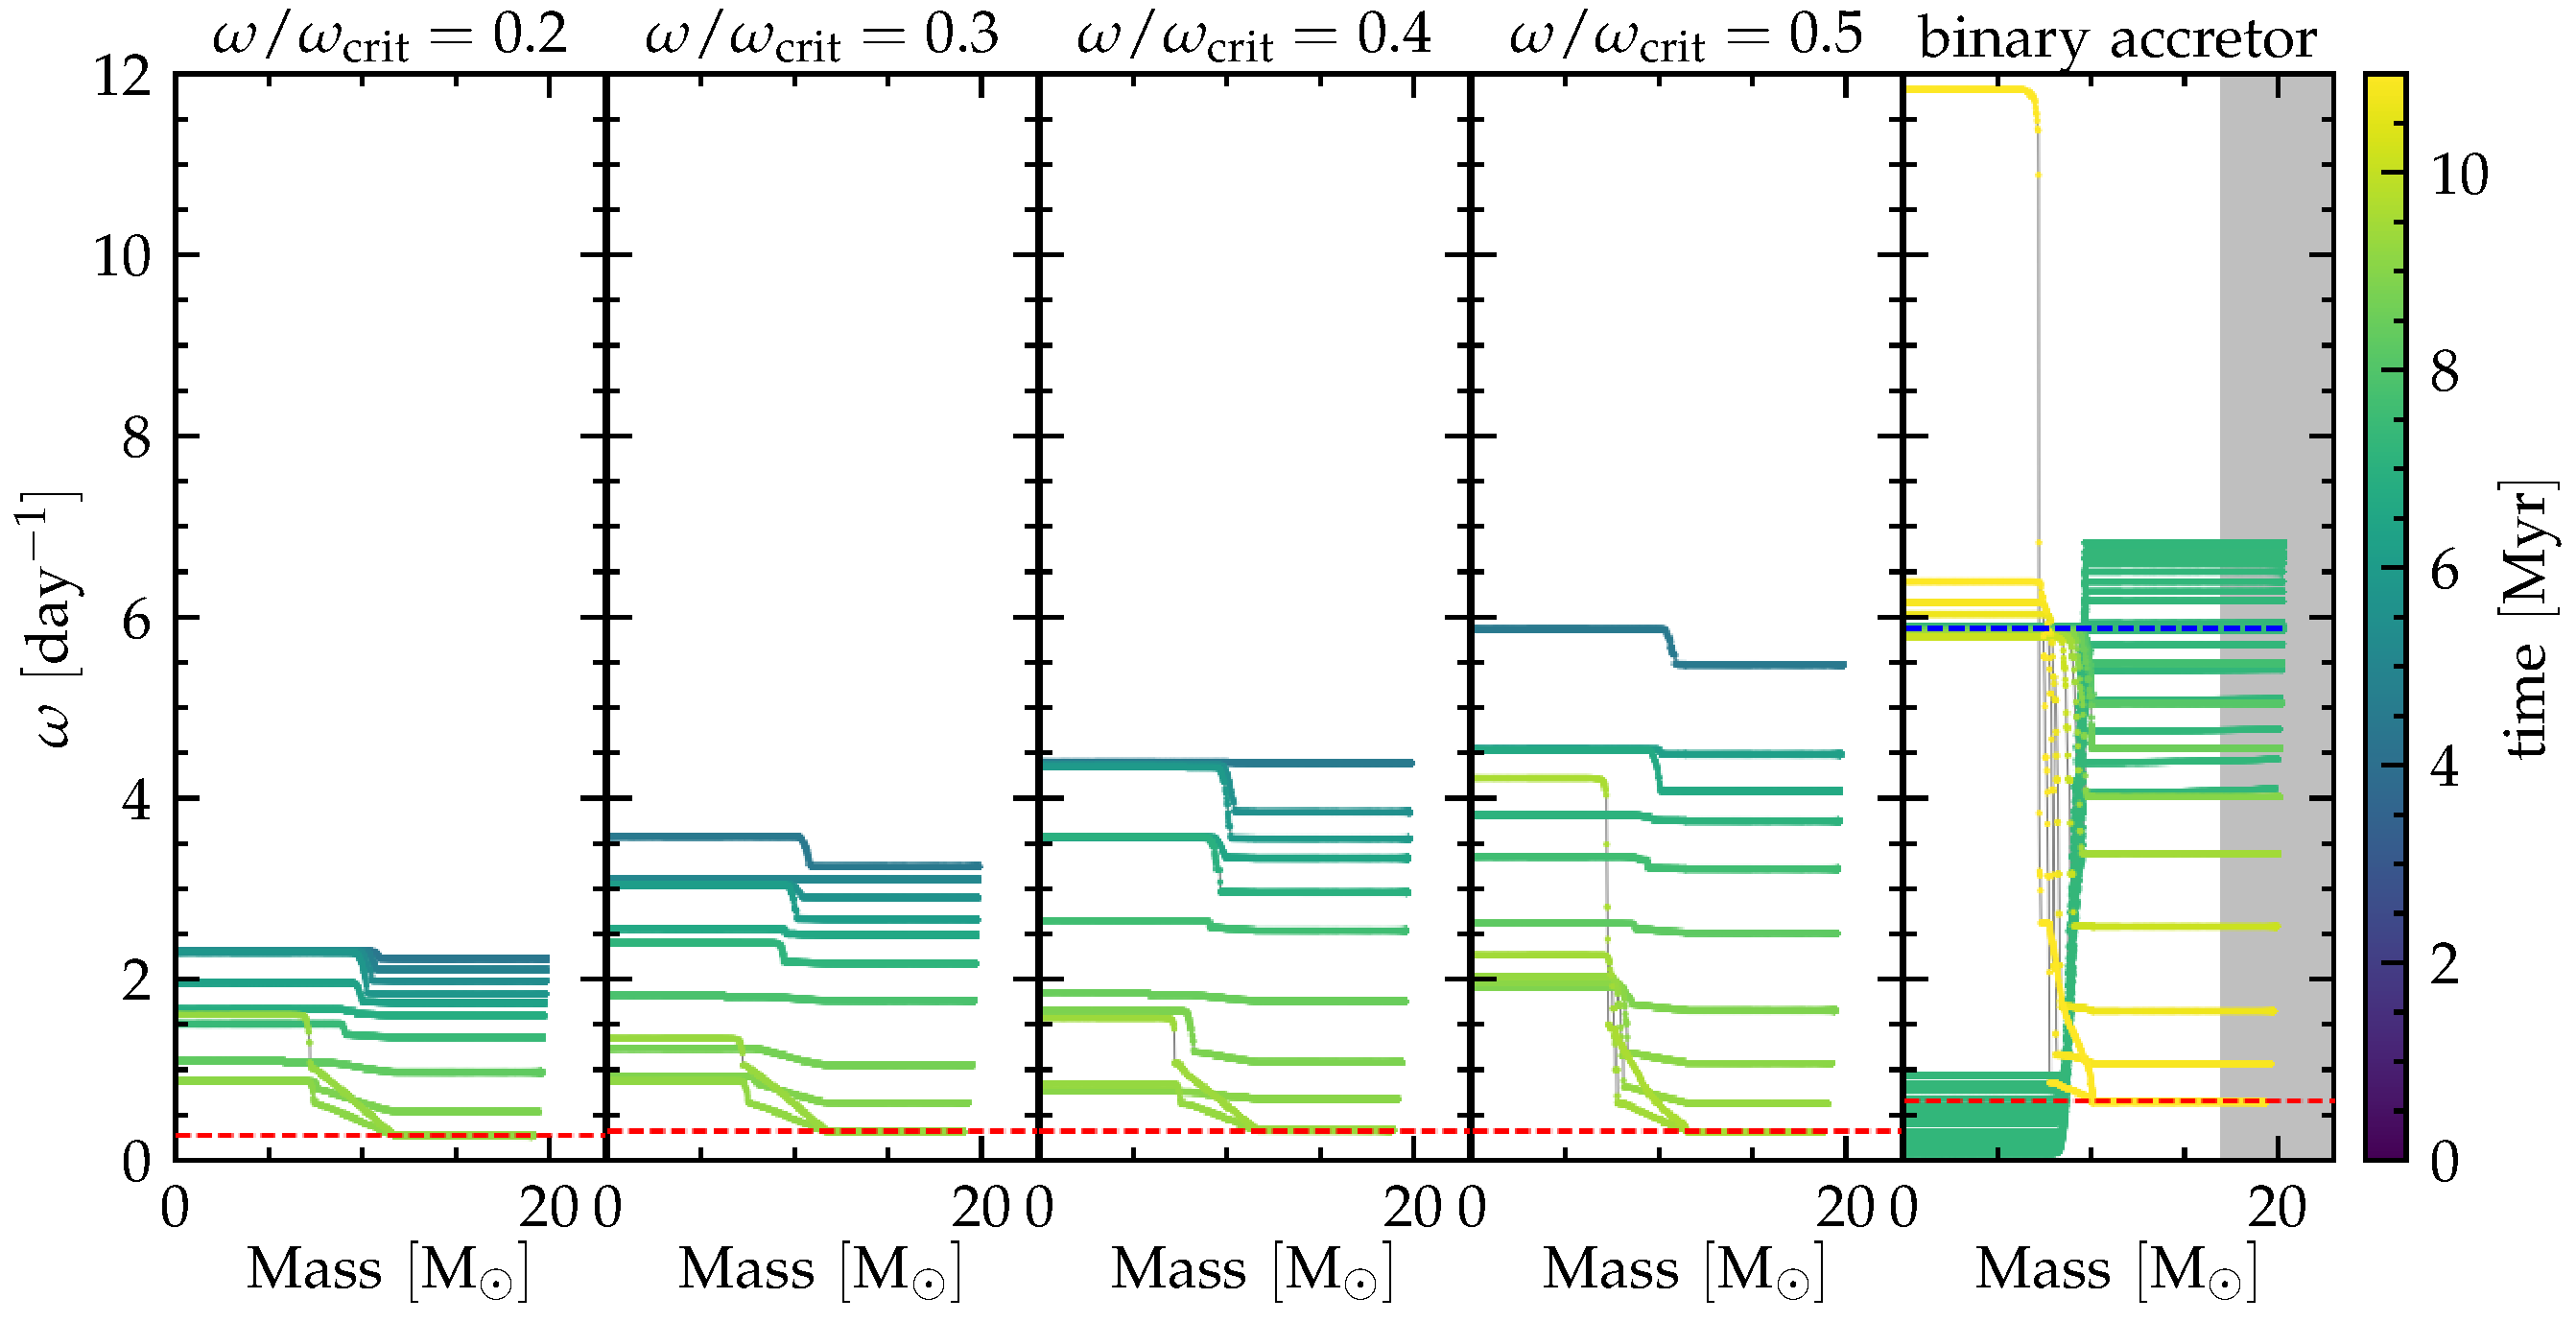
\includegraphics[width=\textwidth]{omega_struct}
  \caption{Top: Internal rotational profile for $20\,M_\odot$ single
    star models with increasing $\omega/\omega_\mathrm{crit}$ at birth
    (first four panels), and for the accretor of our fiducial
    binary. Bottom: internal rotational frequency profile. As in
    \Figref{fig:n14}, the colors go from dark (close to ZAMS) to light
    at TAMS. The dashed black line emphasizes the profile
    corresponding to the blue diamond in \Figref{fig:HRD_both}. In
    the top (bottom) panel the thin dashed red line mark the TAMS surface
    rotation rate (surface rotation frequency). In the rightmost panels, the gray areas indicate
    mass accreted during RLOF. The yellow lines (TAMS) in the last
    panel show that the core of the accretor is rotating almost as
    fast as its surface despite its much smaller radius, and both are
    faster than the surface of single star models.}
  \label{fig:struct_rot}
\end{figure*}

To illustrate the angular momentum transport in our accretor stars, it
is again helpful to compare with single rotating $20\,M_\odot$
models. Typically, single stars are assumed to be solid-body rotators
at ZAMS. Their internal rotational profile evolves differently than
the profile obtained spinning up the secondary star at a later
evolutionary stage, from its surface, and to critical rotation.

The top row of \Figref{fig:struct_rot} shows the internal rotational
velocity $v_\mathrm{rot}=\omega\times r$, while the bottom row shows
the $\omega$ profile. As in \Figref{fig:n14}, the first four panels in
each row show single rotating stars with increasing initial
$\omega/\omega_\mathrm{crit}$, the last panels shows our accretor
model, and the colors go from dark (close to ZAMS) to light
(TAMS). Because of rejuvenation, the accretor has a longer
main-sequence life-time compared to a star of the same final mass,
hence the lighter colors in the last panels (see
\Secref{sec:mix_comparison_single}). The gray area in the rightmost
panels highlights matter accreted during RLOF.

The thin dashed red lines in each panel of the top row of
\Figref{fig:struct_rot} mark the TAMS surface rotation rates: all our
single star models reach a TAMS surface
$v_\mathrm{rot}\simeq50-60\,\kms$. Initially faster rotating models
spin down more in their outer layers, have slightly longer main
sequence lifetimes (because of rotational mixing increasing the
available fuel), and develop stronger differential rotation. As the
core contracts and spins up, the single star profiles show the
progressive development of a core-envelope interface.

Conversely, the last panel shows that the entire interior of the
accretor has a negligible rotational velocity until RLOF (starting at
$7.25$\,Myr). Because of binary interactions, the accretor is spun up
late in its evolution, up to critical rotation
$\omega/\omega_\mathrm{crit}\simeq1$, and from the surface. In our
model, inward transport of angular momentum creates a $v_\mathrm{rot}$
profile monotonically increasing from the center to the surface (green
lines of the last panel in the top row). Late during mass transfer,
the accretor achieves rigid and close to critical rotation (flat
profiles in the last panel on the bottom row of
\Figref{fig:struct_rot}). Rigid rotation\footnote{We define rigid
  rotation with a tolerance of
$\Delta \omega \lesssim 10^{-2}\,\mathrm{days^{-1}}$ between the minimum and maximum
rotational frequency throughout the star.} persists for
$\sim10^{4}$\,years, until and beyond the blue diamond in the bottom
panel of \Figref{fig:HRD_both} where we stop the evolution in a
binary. Afterwards, the accretor's envelope spins down
because of winds. By the end of the main-sequence evolution of the
accretor, the surface still spins with $v_\mathrm{rot}\simeq100\,\kms$
(twice as fast as the single star models).

Perhaps more importantly, the outer-edge of the core has a similar
rotational velocity as the surface, and a much larger rotational frequency than the
cores of single star models. This is because the
evolutionary contraction (decrease in $r$) of the core results in a
significant increase of $\omega$ to conserve the angular momentum that
cannot be efficiently transferred to the outer layers. The core-envelope interface
of the accretor at TAMS is much more prominent than in single rotating
stars. The faster core rotation of binary accretors spun up late and
up to critical rotation might have important implications for the
explosion of the initially less massive star of a binary, the
spin of the resulting compact objects, and the analysis of
gravitational-wave events \citep[e.g.,][]{zaldarriaga:18, qin:18, callister:21}.

\section{Robustness of the models and discussion}
\label{sec:discussion}

Models of the interior evolution of stars require the choice of
several poorly constrained parameters, most arising from the
one-dimensional representation of multi-dimensional phenomena
(convection, mixing, rotation, etc.). This remains true when modeling
two stars in a binary, with the added caveat that an even larger
number of parameters enters in the treatment of binary interactions (and in
particular mass transfer). This emphasizes the need for
observational constraints and motivated us to compare our models to
the observationally well characterized \zoph.

Accretor stars are expected in most populations of (massive)
stars, both in clusters \citep[e.g.,][]{chen:09, wang:20} and in the field
\citep[e.g.,][]{demink:11, demink:13}. However, these might not obviously stand
out as binary products \citep[e.g.,][]{renzo:19walk}. Therefore, to
inform the search for accretor stars in observed samples, it is
also necessary to characterize the robustness of model predictions
against numerical, physical, and algorithmic choices.

In \Secref{sec:single_star_uncertainties}
we report on exploration of parameter variations for each individual
star in the binary. We discuss parameters governing the mass transfer phase in
\Secref{sec:bin_param}, the initial binary architecture in
\Secref{sec:bin_init}, and the consequences of the assumed SN
explosion of the companion in \Secref{sec:SN_comp}.


\subsection{Uncertainties in the single-star physics}
\label{sec:single_star_uncertainties}
% rotation
Rotation is a critical ingredient of our models: it governs the
equatorial radius and thus $\omega/\omega_\mathrm{crit}$, therefore by
assumption it also controls the mass transfer efficiency through
mechanical enhancement of the accretor's wind (see
\Secref{sec:bin_param}). Through Eddington-Sweet meridional
circulations, rotation determines outward mixing from the core, and
more importantly inward mixing from the surface.  We emphasize that
the shellular approximation used in one-dimensional stellar evolution
codes might not be appropriate for
$\omega/\omega_\mathrm{crit}\simeq 1$ reached by our accretor star
during RLOF. Decreasing by a factor of 10 the diffusion coefficient
for Eddington-Sweet meridional circulations has a very small effect on
the evolution of the accretor on the HR diagram. However, the noisiness during the
late RLOF phase (beyond point B in \Figref{fig:HRD_both}) increases in
amplitude, confirming that the details of this part of the evolution
are sensitive to the treatment of rotational mixing (and its interplay
with other processes). % We were unable to run models turning completely
% off Eddington-Sweet meridional circulations past the ``kink'' feature
% in \Figref{fig:HRD_both}.

Our models assume a Spruit-Tayler dynamo \citep{spruit:02} for the
transport of angular momentum throughout the evolution. Adopting the
stronger angular momentum transport from \cite{fuller:19} might result
in a more efficient spin-down of the surface during RLOF, possibly
allowing for more accretion of mass.

The accretor is spun up late, from the surface inwards, and to
critical rotation compared to single star models which are initialized
at ZAMS with rigid rotation. Late during the mass transfer, even the
weaker core-envelope coupling of \cite{spruit:02} is sufficient for
the accretor to achieve rigid rotation. Subsequently, the envelope
spins down because of wind mass loss and more importantly the core
spins significantly up because of its evolutionary contraction. We
expect that following \cite{fuller:19} the core would lose more
angular momentum to the envelope, limiting its ability to spin up as
it contracts and decreasing its rotational velocity.
Nevertheless, we expect that the difference with single star
rotational profiles would remain because of the shorter evolutionary time left.

% thermohaline mixing
During RLOF, thermohaline mixing in the envelope also becomes
important. In \MESA, each mixing process is represented by its own
diffusion coefficient, and they are then summed together
\citep[e.g.,][]{paxton:11}, under the implicit assumptions that mixing
processes are independent from each other. This is typically
reasonable since locally one process dominates the mixing.

In the envelope of our accretor model, initially Eddington-Sweet circulations are
dominant, however thermohaline mixing reaches and exceeds their
diffusivity late during the mass transfer. If fast rotation can
physically modify thermohaline mixing processes, this might impact our
accretor models.  We also tried models enhancing the efficiency of
thermohaline mixing by a factor of 100 \citep{schootemeijer:19} but
these proved numerically unstable when accreting CNO-processed material.

We have also explored models with a step overshooting following
\cite{brott:11}. Our fiducial exponential overshooting was chosen to
reproduce the width of the main-sequence of the models of
\cite{brott:11}, and not-surprisingly, the qualitative evolution of
our fiducial model and our models with step overshooting is
similar. However, adopting a step overshooting provides a higher
diffusivity at the outer edge of the core which ultimately impacts the
details of the chemical profile at the outer edge of the core, and the
morphology of the evolutionary tracks during late RLOF.

% weak wind
\zoph\ is one of the low-luminosity O-type stars for which
\cite{marcolino:09} found a lower-than-predicted mass loss rate.
To address the ``weak wind problem'', we also attempted
running models with artificially decreased wind mass loss rate
\citep[e.g.,][]{renzo:17}, but these resulted in super-critical
$\omega/\omega_\mathrm{crit}>1$ post-RLOF accretor stars with untrustworthy
numerical results.

%metallicity
Our model presented in \Secref{sec:best_model}, assumes an initial
metallicity $Z=0.01$ informed by the asteroseismology of low mass
stars in the parent association Upper-Centaurus-Lupus
\citep[e.g.,][]{murphy:21}. Moreover, we have assumed that mass
fractions of each element scale with the Solar values
\citep{grevesse:98}, which might not be appropriate especially for
massive stars \citep[e.g.,][]{grasha:21}. With these assumptions, the
initial mass fraction of $^{12}\mathrm{C}$ and $^{14}\mathrm{N}$ are
lower than the values for \zoph\ reported by
\citetalias{villamariz:05}. Even though their surface values increase
during mass transfer, our model still slightly under-predicts
them. Improved agreement could be obtained changing the ratio of
abundances to non-solar values, or by changing the efficiency of
downward rotational and thermohaline mixing which dilutes the accreted
material into the secondary's envelope.

We also run a model identical to the one described in
\Secref{sec:best_model}, except with $Z=Z_\odot=0.0142$
\citep{asplund:09}. Qualitatively, the binary evolution remains
similar, with the higher metallicity stars having slightly larger
radii and cooler $T_\mathrm{eff}$ at a given luminosity. This still
produces a stable case B RLOF, however, the accretor track is
displaced on the right on the HR diagram. Thus, matching the high present-day
$T_\mathrm{eff}=32\,000\pm2\,000$ of \zoph\ (e.g., \citetalias{villamariz:05}) requires more
massive and hotter accretors at higher $Z$ (see also \Secref{sec:bin_init}).

% While the number of free parameters resulting in a successful
% computation is rather limited, we emphasize that this remains often
% true for calculation of single massive star evolution.

\subsection{Uncertainties in the treatment of mass transfer}
\label{sec:bin_param}

We regulate the accretion efficiency through the rotational
enhancement of mass loss \citep[e.g.,][]{langer:98}.
However, whether critical rotation can effectively stop the accretion
of matter is unclear. \cite{popham:91} and \cite{paczynski:91}
argued that accretion of mass (but not angular momentum) might be
possible even at or beyond critical rotation.

During RLOF, the total amount of mass lost by the donor is
$\Delta M_\mathrm{donor} \simeq 10.6\,M_\odot$, of which only
$\Delta M_\mathrm{accretor}\simeq 3.4\,M_\odot$ are successfully
accreted by the companion. This corresponds to an overall mass transfer efficiency
$\beta_\mathrm{RLOF}\equiv |\Delta M_\mathrm{accretor}|/|\Delta M_\mathrm{donor}| \simeq 0.32$,
although the accretion efficiency is \emph{not} constant throughout
the mass transfer \citep[e.g.,][]{vanrensbergen:06}. In our models,
the mass transfer efficiency depends on the radial and rotational
evolution of the accreting star. During RLOF, the accretor is out of
gravothermal equilibrium with significant impact on its radius and
ultimately on the amount of mass transferred and its angular
momentum. In reality, the gas stream between the two stars, the
hot-spot due to the RLOF stream hitting the accretor's surface (see below), and
the geometric distorsion of the outer layers because of the
centrifugal forces would not follow the spherical symmetry imposed by
1D codes such as \texttt{MESA}.

While the mass transfer efficiency $\beta_\mathrm{RLOF}$ and
importantly its time-evolution need further attention, it is also
likely that this parameter and its evolution depend on the details of
the system (masses, mass ratio, period, etc.). For instance, to
explain the lower mass sdO+Be binaries found by \cite{wang:21_sdOBe} it is likely
that a larger mass transfer efficiency would be required.


We emphasize that most studies, especially using rapid population
synthesis tools, typically assume a constant $\beta_\mathrm{RLOF}$ and
neglect to model the out-of-equilibrium phase of the accretor and how
this can impact the binary and orbital evolution. Alternatively, rapid
population synthesis can limit the accretion rate based on the thermal
timescale of the accretor (calculated from models in gravothermal
equilibrium). Based on this approach, \cite{schneider:15} found a
higher $\beta_\mathrm{RLOF}\simeq 0.7$ for a binary comparable to ours
(initially $M_1=20\,M_\odot$, $M_2=0.7M_1$ with separation
$a\simeq300\,R_\odot$), although their $\beta_\mathrm{RLOF}$ is very
sensitive to the initial mass ratio and period in this regime.

Another free parameter in the treatment of mass transfer is the
specific angular momentum of the accreted material. This is an
uncertain quantity and likely depends on the geometry of the accretion
process, and in particular, whether the accretion stream through the
L1 Lagrangian point hits directly the accretor star, or if
instead an accretion disk is formed \citep[e.g.,][]{demink:13}.

We calculate the minimum distance $R_\mathrm{min}$ between the stream
coming from the L1 Lagrangian point and the accretor using the fit
from \cite{ulrich:76} to the numerical results of \cite{lubow:75}. We
find $R_\mathrm{min}\simeq 1.5\,R_\odot < R_\mathrm{accretor}$: this
suggests that the stream should directly hit the accretor, without
forming an accretion disk. Nevertheless, for the sake of numerical
stability, we assume the incoming material and the stellar surface to
have the same specific angular momentum. This provides a slow angular
momentum accretion and consequent spin-up of the surface.

We also attempted calculations using for specific angular momentum of
the incoming material $\sqrt{1.7GM_\mathrm{accretor}R_\mathrm{min}}$
\citep{lubow:75} for direct impact of the incoming stream with the
accretor. This is typically much larger than
the specific angular momentum of the accretor's surface. However,
these models proved numerically more unstable and providing less
trustworthy results after the accretor is spun up
significantly. In general, allowing for a faster accretion of
angular momentum results in less radial expansion of the accretor
(cf.~\Figref{fig:HRD_both}), faster spin-up, and a lower overall mass
transfer efficiency $\beta_\mathrm{RLOF}$.

In our models, the composition of the transferred material is
determined by the structure of the donor and the mass transfer rate
calculated following \cite{kolb:90}, but we need to specify its
specific entropy when it reaches the accretor surface. We follow the
common practice of assuming the specific entropy of the incoming
material to be same as the accreting surface. The scenario justifying
this hypothesis is that during RLOF the matter is
sufficiently optically thin so that radiative processes can rapidly
equalize the entropy between the RLOF stream and the accreting
surface. However, the very large mass-transfer rates we find
(cf.~\Figref{fig:MT}) might result in optically thick flows for which
this approximation might not be appropriate.

Because of the increase in mass, our accretor star is rejuvenated: its
total main-sequence lifetime is longer than the lifetime of a single
star born with the final post-RLOF mass of the accretor\footnote{But
  not longer than the lifetime of a single star of its initial,
  pre-RLOF mass.}
\citep[e.g.,][]{schneider:16}. The rejuvenation is due to the increase
- in mass - of the core region, which brings inward fresh
nuclear fuel. Our results are in agreement with \cite{hellings:83},
while \cite{braun:95} did not find any rejuvenation in their accretor
models. We attribute this difference to the lack of convective
boundary mixing (e.g., overshooting, efficient semiconvection, shear)
in their models, which impedes the growth of the core.

\begin{figure}[htbp]
  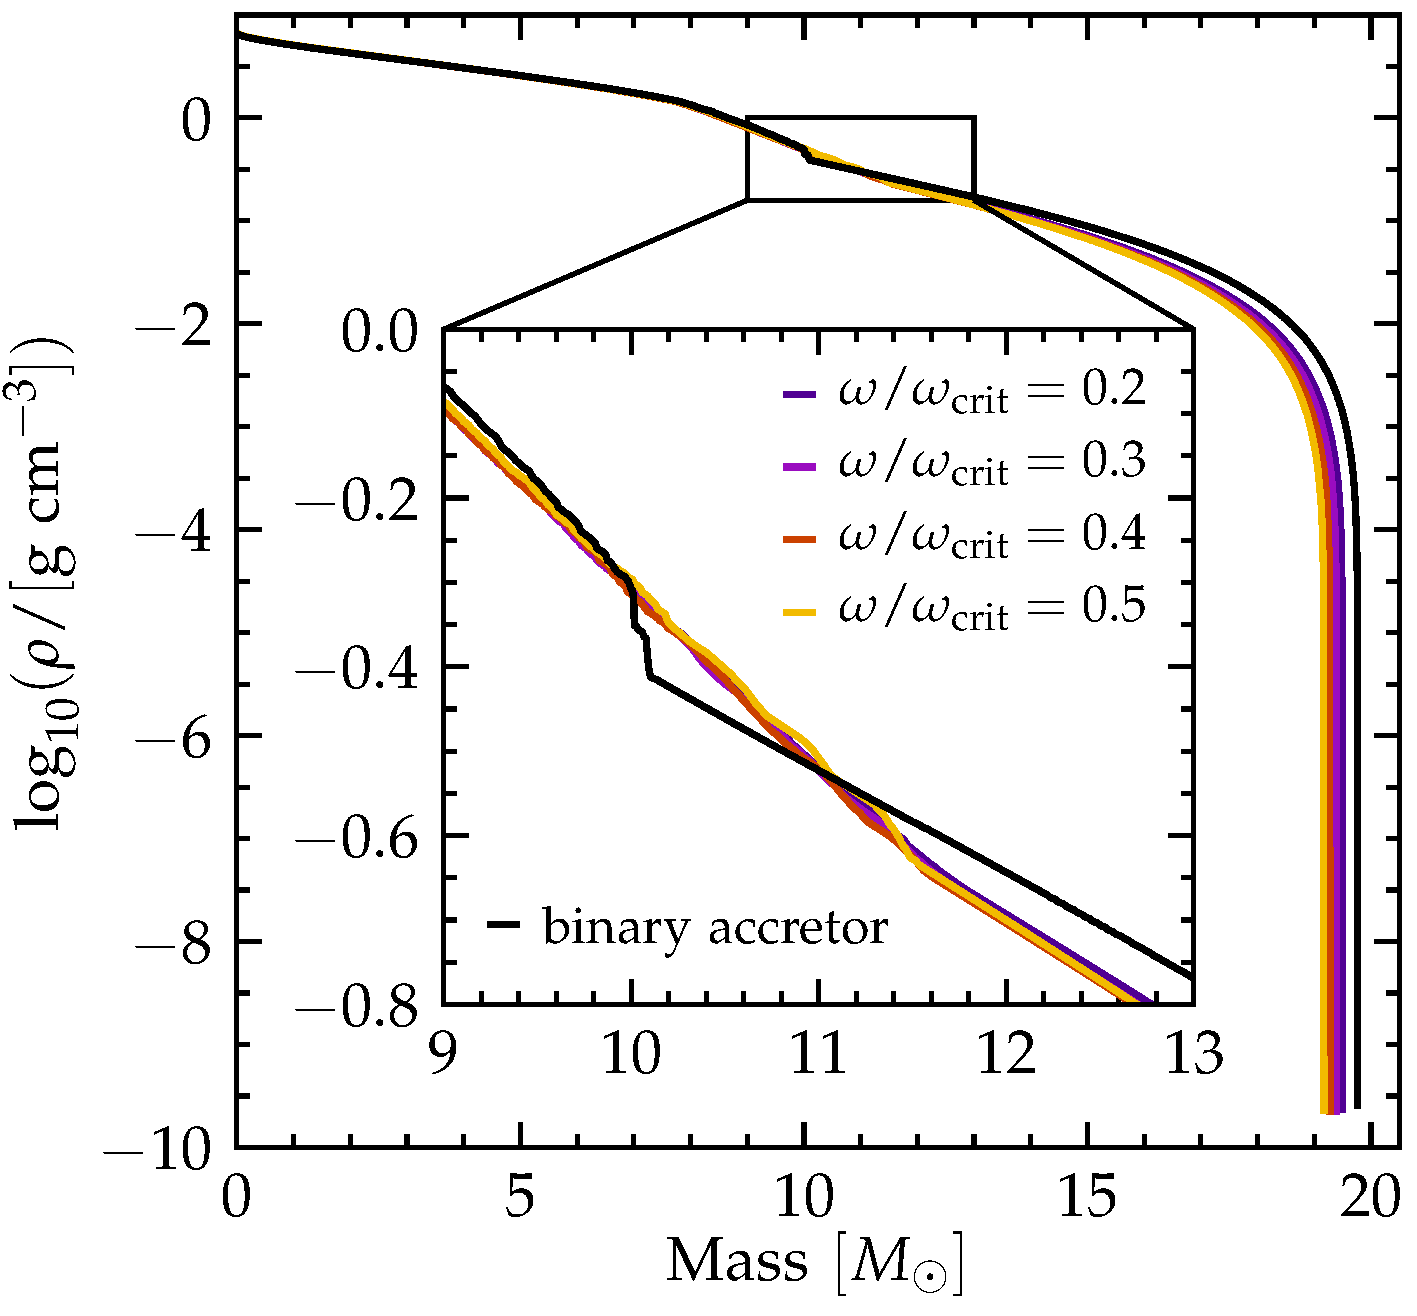
\includegraphics[width=0.47\textwidth]{rho_comparison}
  \caption{Comparison of the density profiles of the accretor model
    (black) and single $20\,M_\odot$ rotating stars (colors). The models are
    compared when they reach the same central H mass fraction of
    $X_c=0.085$ (point G in \Figref{fig:HRD_both} for the accretor). The inset magnifies the region above the core, where the outcome of common envelope events is
    decided. Because of the growth of the core, the density profile of
  the accretor in this region is significantly different.}
  \label{fig:rho}
\end{figure}

In our models, the growth of the core is initially driven by
convection and overshooting, and to a lesser extent to dynamical
shear. Later on, a convective region above the overshooting region
develops (third panel onwards in \Figref{fig:D_mix}) and remains as an off-center feature until and beyond point G
in \Figref{fig:HRD_both}.

\Figref{fig:rho} shows a density comparison between the accretor in
the last panel of \Figref{fig:D_mix} and four initially $20\,M_\odot$
single rotating stars. The off-center convective region significantly
alters the density profile above the core of the accretor compared to
a single star. The sharper inner density drop and shallower density
profile of accretors might be probed with asteroseismology: \zoph\
itself has been observed to show non-radial pulsations
\citep{walker:05}, which may be involved in the transient appearance of
emission lines and a decretion disk. If compared to a star of comparable mass which
evolved as single, the pulsations could shed light on the structural
differences between single stars and binary products.

Moreover, if the binary system remains bound after the explosion of
the companion and the evolutionary expansion of the accretor leads
to a common envelope \citep[e.g.,][]{paczynski:76}, the layer above
the He core is crucial to determine the success or failure of the
common envelope ejection. Although this is not the future fate of
\zoph, this might be crucial for our understanding of gravitational
wave progenitors.  Common envelope simulations have so far
neglected the impact of previous RLOF phase(s) on the density
structure of the stars initiating the dynamically unstable mass
transfer.

\subsection{Variations in initial binary parameters}
\label{sec:bin_init}

The initial donor mass $M_1$, mass ratio $q=M_2/M_1$, and the period
of the progenitor binary of \zoph\ cannot be directly constrained from
observations. We have explored variation in these values, and the
qualitative behavior of the models is similar.
Shorter initial periods results in larger post-RLOF orbital
velocities, and thus larger runaway velocities if the binary is
disrupted at the first SN (see \Secref{sec:SN_comp}). For example, taking $P$=75\,days
(cf.\ 100\,days in our fiducial model in \Secref{sec:best_model}), the
binary still experiences stable case B mass transfer, but the
post-RLOF orbital velocity of the accretor is about $60\,\kms$, that
is $\sim$$10\,\kms$ higher
than in our fiducial model.

Increasing the donor mass also has a similar effect on the post-RLOF orbital velocity of the accretor. Using
$M_1=30\,M_\odot$ (cf.\ $25\,M_\odot$ in \Secref{sec:best_model}),
$M_2=17\,M_\odot$, and
$P$=100\,days, we obtain a post-RLOF velocity of
$65\,\kms$. However, this produces a stripped donor of
$\sim$16\,$M_\odot$ at RLOF detachment, with stronger wind mass loss. Therefore this binary is expected to widen relatively more than our fiducial model of \Secref{sec:best_model}, slowing down the secondary. The increased mass of the stripped star could also imply a lower chance of exploding for the donor, which might instead collapse to a black-hole instead (however, see \Secref{sec:SN_comp}).

The higher $M_1$ does not significantly change the post-RLOF total
mass of the accretor, with $M_2$ remaining about $\sim$20.5\,$M_\odot$, since
in our models accretion is regulated mostly by the spin up of the
accretor, and we do not couple the specific angular momentum of the transferred
material to the orbit or the donor's spin.

However, changing the initial mass ratio also changes the difference
between the main-sequence lifetime of the two stars, and thus how far
along the main sequence the accretor is at the onset of RLOF. The observed
position of \zoph\ on the HR diagram, particularly its relatively high
$T_\mathrm{eff}$ are difficult to reproduce assuming initially less
massive accretors (which would remain too cool even after accreting
mass), or more equal initial mass ratio (which would produce an
accretor that is too evolved and cool at the onset of mass transfer).

\subsection{The explosion of the donor star}
\label{sec:SN_comp}

Throughout this study, we have assumed the ``binary SN scenario'' to
explain the runaway nature of \zoph:
after the mass transfer phase, the explosion of the donor disrupts the
binary and ejects the accretor at roughly its pre-explosion orbital
velocity \citep[e.g.,][]{renzo:19walk}. This fate occurs to the
majority of massive binary systems, and \zoph\ might be the best
example of it \citep[e.g.,][]{blaauw:52, blaauw:61,
  hoogerwerf:00}. \cite{neuhauser:20} suggested not only the companion
successfully exploded producing the pulsar PSR B1706-16 and ejecting
\zoph, but also that the
explosion produced radioactive $^{60}\mathrm{Fe}$ which polluted
Earth.

From kinematic and orbital considerations they estimated the pulsar
received a natal kick of
$253\pm54\,\kms$, which would be sufficiently large to unbind the
binary which has $v_\mathrm{orb}=\sqrt{G(M_1+M_2)/a}\simeq 135\,\kms$
at the end of our binary simulation (blue diamond in \Figref{fig:HRD_both}) and this will decrease further in the
remaining time to the donor's core-collapse \citep{kalogera:96,
  tauris:15}.

The SN ejecta mass would depend on the post-RLOF wind mass loss of our
donor star, which is very uncertain \citep[e.g.,][]{renzo:17, vink:17,
  gilkis:19}.  At the end of our binary evolution simulation, our
stripped donor is
$\sim$$9.4\,M_\odot$, with a surface H fraction of
$X\lesssim0.2$ for a layer of $\Delta M \simeq
2.5\,M_\odot$.  Its wind mass-loss rate is $\sim10^{-5}\,M_\odot \
\mathrm{yr^{-1}}$ (cf.~\Figref{fig:MT}), likely to increase as it contracts and increases its luminosity and effective temperature. We expect its explosion to appear as H-less type Ib SN. Although our stripped donor is rather massive, recent studies hints at a higher ``explodability'' of donor stars in binary systems \citep[e.g.,][]{schneider:21, laplace:21, vartanyan:21}.

We have neglected the impact of the explosion on the structure of the accretor star. At the time of the explosion, the accretor subtends a solid angle
$\sim$$R^2/a^2\simeq 2\times10^{-3}$\,steradians with $R$ the accretor
radius and $a$ the binary separation. We neglect the post-RLOF
wind-driven orbital widening for this estimate.  The blast wave will
hit the accretor causing mass loss -- directly via ablation and by
injecting energy in the envelope, inflating it and enhancing its wind
\citep{wheeler:75, tauris:98, podsiadlowski:03, hirai:18}.  Because of
the SN shock, the just ejected new runaway star might appear bloated
and redder (long before it overtakes the slowing SN remnant). The
impact of this brief out of thermal equilibrium phase on the stellar
spin should be investigated further.

Using 2D hydrodynamic simulations of the star-SN ejecta interactions in close binaries ($a\lesssim
60\,R_\odot$, cf. $a\gtrsim
343\,R_\odot$ in our fiducial binary model), \cite{hirai:18} found that the companion star recovers its pre-explosion luminosity and effective temperature within a few years to decades, and the amount of mass removed by the SN shock is
$\lesssim10^{-2}\,M_\odot$.  The SN ejecta might also pollute the surface of the runaway depositing processed nuclear material \citep[e.g.,][]{przybilla:08, suda:21}. However, for the large final separation of our model, little pollution is expected and enhahnced mass loss and inward mixing might quickly dilute any signature below detectable levels.

\section{Summary \& conclusions}
\label{sec:conclusions}

So far, the impact of mass transfer on the structure and evolution of accretor in massive
binaries has received little attention.  To investigate this, we have
ran \texttt{MESA} calculations of massive binaries evolving two
coupled stars simultaneously.

As a first application, we focused on finding a model qualitatively
matching observations of the nearest O-type star to Earth. This is the
runaway \zoph, which has long been suggested to be a former accretor
star ejected from a binary at the core-collapse of the
companion \citep[binary SN scenario,][]{blaauw:61}. However, our
models are also informative for the generic population of massive
accretors.

\subsection{Reproducing \zoph}

We found that the main features of \zoph\ can be
reasonably well reproduced using standard stellar physics
assumptions for the treatment of mass transfer, chemical mixing, and
rotation. Our choices are described in \Secref{sec:methods} and
Appendix~\ref{sec:software}.

Our fiducial model is a binary starting
with $M_1=25\,M_\odot$, $M_2=17\,M_\odot$, and $P=100$\,days at
metallicity $Z=0.01$ (see \Secref{sec:best_model}). This binary
experiences stable thermal-timescale Roche lobe overflow after the end
of the main sequence of the donor (case B).

The accretor
compares rather well with observations of \zoph\ about $1.5-2$\,Myrs
after the end of mass transfer, corresponding to the remaining donor's
lifetime at the end of our simulations plus the kinematic age of
\zoph. Specifically, the position on the HR diagram, the runaway space
velocity (estimated based on the accretor's orbital velocity), the
surface composition and rotational velocity are in the right ballpark.

Our model of \zoph\ differs significantly from previous studies: in
contrast with the accretor models of \cite{vanrensbergen:96}, in our
model the $^{14}\mathrm{N}$- and $^4\mathrm{He}$-rich surface
composition is not the result of pure outward rotational mixing.
Instead, this material is transferred from the receeding core of the
donor star and mixed from the surface inwards into the accretor by
meridional circulations and thermohaline mixing.  Thus, the present
day surface mass fractions of \zoph\ put a coupled constrain the mass
transfer efficiency and mixing in the accretor. \zoph\ should
\emph{not} be used to calibrate models of rotational mixing in single
star models.

We emphasize that the surface composition alone would not be a
smoking-gun, especially given the large uncertainties in the treatment
of rotation and mixing in stellar evolution models. In our models, the
accretion of $^{14}\mathrm{N}$ from the donor allows the accretor to
be simultaneously fast rotating and $^{14}\mathrm{N}$-rich, while
single rotating stars can only mix upward $^{14}\mathrm{N}$ from their
core, and have significantly spun down by the time they become
$^{14}\mathrm{N}$-rich. Moreover, alternative scenarios where \zoph\
evolved as a single fast-rotating star require ad-hoc explanations for the runaway velocity,
and have been shown by \citetalias{villamariz:05} to struggle in reproducing
surface mass fractions, apparent age, mass, and rotation rate simultaneously.

The surface rotation rate of the accretor post-mass-transfer is always
higher than the rotation rate of single stars initialized with
half-critical rotation, but might still be on the low side compared to
\zoph. However, the wind spin down might be overestimated in our
models (weak wind problem).

We also tested the
robustness of this model against variations in the initial parameters
and algorithmic representation of physical phenomena, discussed in
\Secref{sec:discussion}. Less massive accretors remain too cool
throughout the evolution to be compatible with \zoph, and more equal
initial mass ratios lead to a more evolved accretor at the onset of
mass-transfer, again resulting in too cool temperatures. Increasing
the donor's initial mass might result in stripped stars unlikely to
form a neutron star in their final SN explosion.

\subsection{Accretors are not  single rotating stars}

Our models also highlight some general differences between accretors in massive
binaries and stars evolving as single throughout their life. These
have been so far under-appreciated but might be important for several
sub-fields of astrophysics, including asteroseismology, stellar
populations, and time-domain and gravitational waves observations.

The first notable difference we find is the internal rotation
profile. Single rotating stars are usually initialized as rigid
rotators at birth, and throughout their evolution they spin down to
wind mass loss. Conversely, accretors are spun up later (roughly
half-way through the main sequence in our model from
\Secref{sec:best_model}), and from the surface. Moreover, for single
stars the maximum rotation rate, that is the one assumed at the
beginning of the evolution, is a poorly constrained parameter
\citep[e.g.,][]{ramirez-agudelo:13, ramirez-agudelo:15}. Conversely,
accretors in binaries reach critical rotation
$\omega/\omega_\mathrm{crit}\simeq 1$.  The later spin-up and higher
rotation achieved allow the accretor star to remain a fast rotator
until the end of its main sequence.

The angular momentum accreted at the surface of the accretor is
transported into the core (by the Spruit-Tayler dynamo in our
simulations). This results in a much faster rotating helium core at the end
of the main sequence compared to single stars, with potential
implications for the final explosion and the resulting compact object
born from the accretor star in an interacting binary system.

Finally, in our models, the accretion of mass and consequent
rejuvenation of the accretor leads to a different density profile at
the bottom of the envelope. The details of the difference are likely
sensitive to what allows the core to grow and the rejuvenation to
happen. In our models,
the growth of the core leads to an off-center convective shell (cf.\
\Figref{fig:D_mix} and \Figref{fig:rho}). This shell results in a
sharper density drop at the core edge, and a flatter density profile
close to the end of the main sequence. This could in principle be
probed by asteroseismology. Depending on how the accretor (and the
binary) evolves in the future, this difference could be crucial in
determining the outcome of common envelope events between massive
stars and compact objects.\\


Improving our understanding of the evolution of the initially less
massive stars in massive binary systems is crucial for the upcoming
large surveys, stellar kinematics,  and for the understanding of the evolution of
gravitational-wave progenitors in isolated binaries. Although
presently single, the nearest O-type star to Earth, \zoph, can be used
as an anchor point for the modeling of accretors. Our models
demonstrate that a broad agreement with observations can be
achieved with standard stellar evolution assumptions. Future efforts
should extend these models to a wider mass, period, mass ratio, and metallicity
range to investigate the impact of binary evolution on the life,
explosion, and after-life of the secondary stars in massive binary
systems.

\software{
  \MESA\ \citep{paxton:11,paxton:13,paxton:15,paxton:18,paxton:19},
  \texttt{mesaSDK} \citep{mesasdk},
  \texttt{ipython/jupyter} \citep{ipython},
  \texttt{matplotlib} \citep{matplotlib},
  \texttt{mesaPlot} \citep{mesaplot},
  \texttt{NumPy} \citep{numpy}.
}
\acknowledgements{We are grateful to E.~Zapartas, A.~Jermyn,
  M.~Cantiello, and R.~Neuh\"auser for helpful discussions.}

\appendix

\section{\texttt{MESA} setup}
\label{sec:software}

We use \code{MESA} version 15140 to compute our models.  The
\code{MESA} equation of state (EOS) is a blend of the OPAL \citet{Rogers2002}, SCVH
\citet{Saumon1995}, PTEH \citet{Pols1995}, HELM \citet{Timmes2000},
and PC \citet{Potekhin2010} EOSes.

OPAL \citep{Iglesias1993, Iglesias1996} provides the main radiative
opacities, with low-temperature data from \citet{Ferguson2005} and the
high-temperature from \citet{Buchler1976}. Electron conduction
opacities are from \citet{Cassisi2007}.

Nuclear reaction rates are a combination of rates from NACRE
\citep{Angulo1999}, JINA REACLIB \citep{Cyburt2010}, plus additional
tabulated weak reaction rates \citet{Fuller1985, Oda1994,
  Langanke2000}. Screening is included via the prescription of
\citet{Chugunov2007}.  Thermal neutrino loss rates are from
\citet{Itoh1996}. We use a
22-isotope nuclear network (\texttt{approx\_21\_plus\_cr56}).

The inlists, processing scripts, and model output are available at~\todo{zenodo}.

\section{Resolution tests}
\label{sec:res_tests}


\begin{figure*}[htbp]
  \centering
  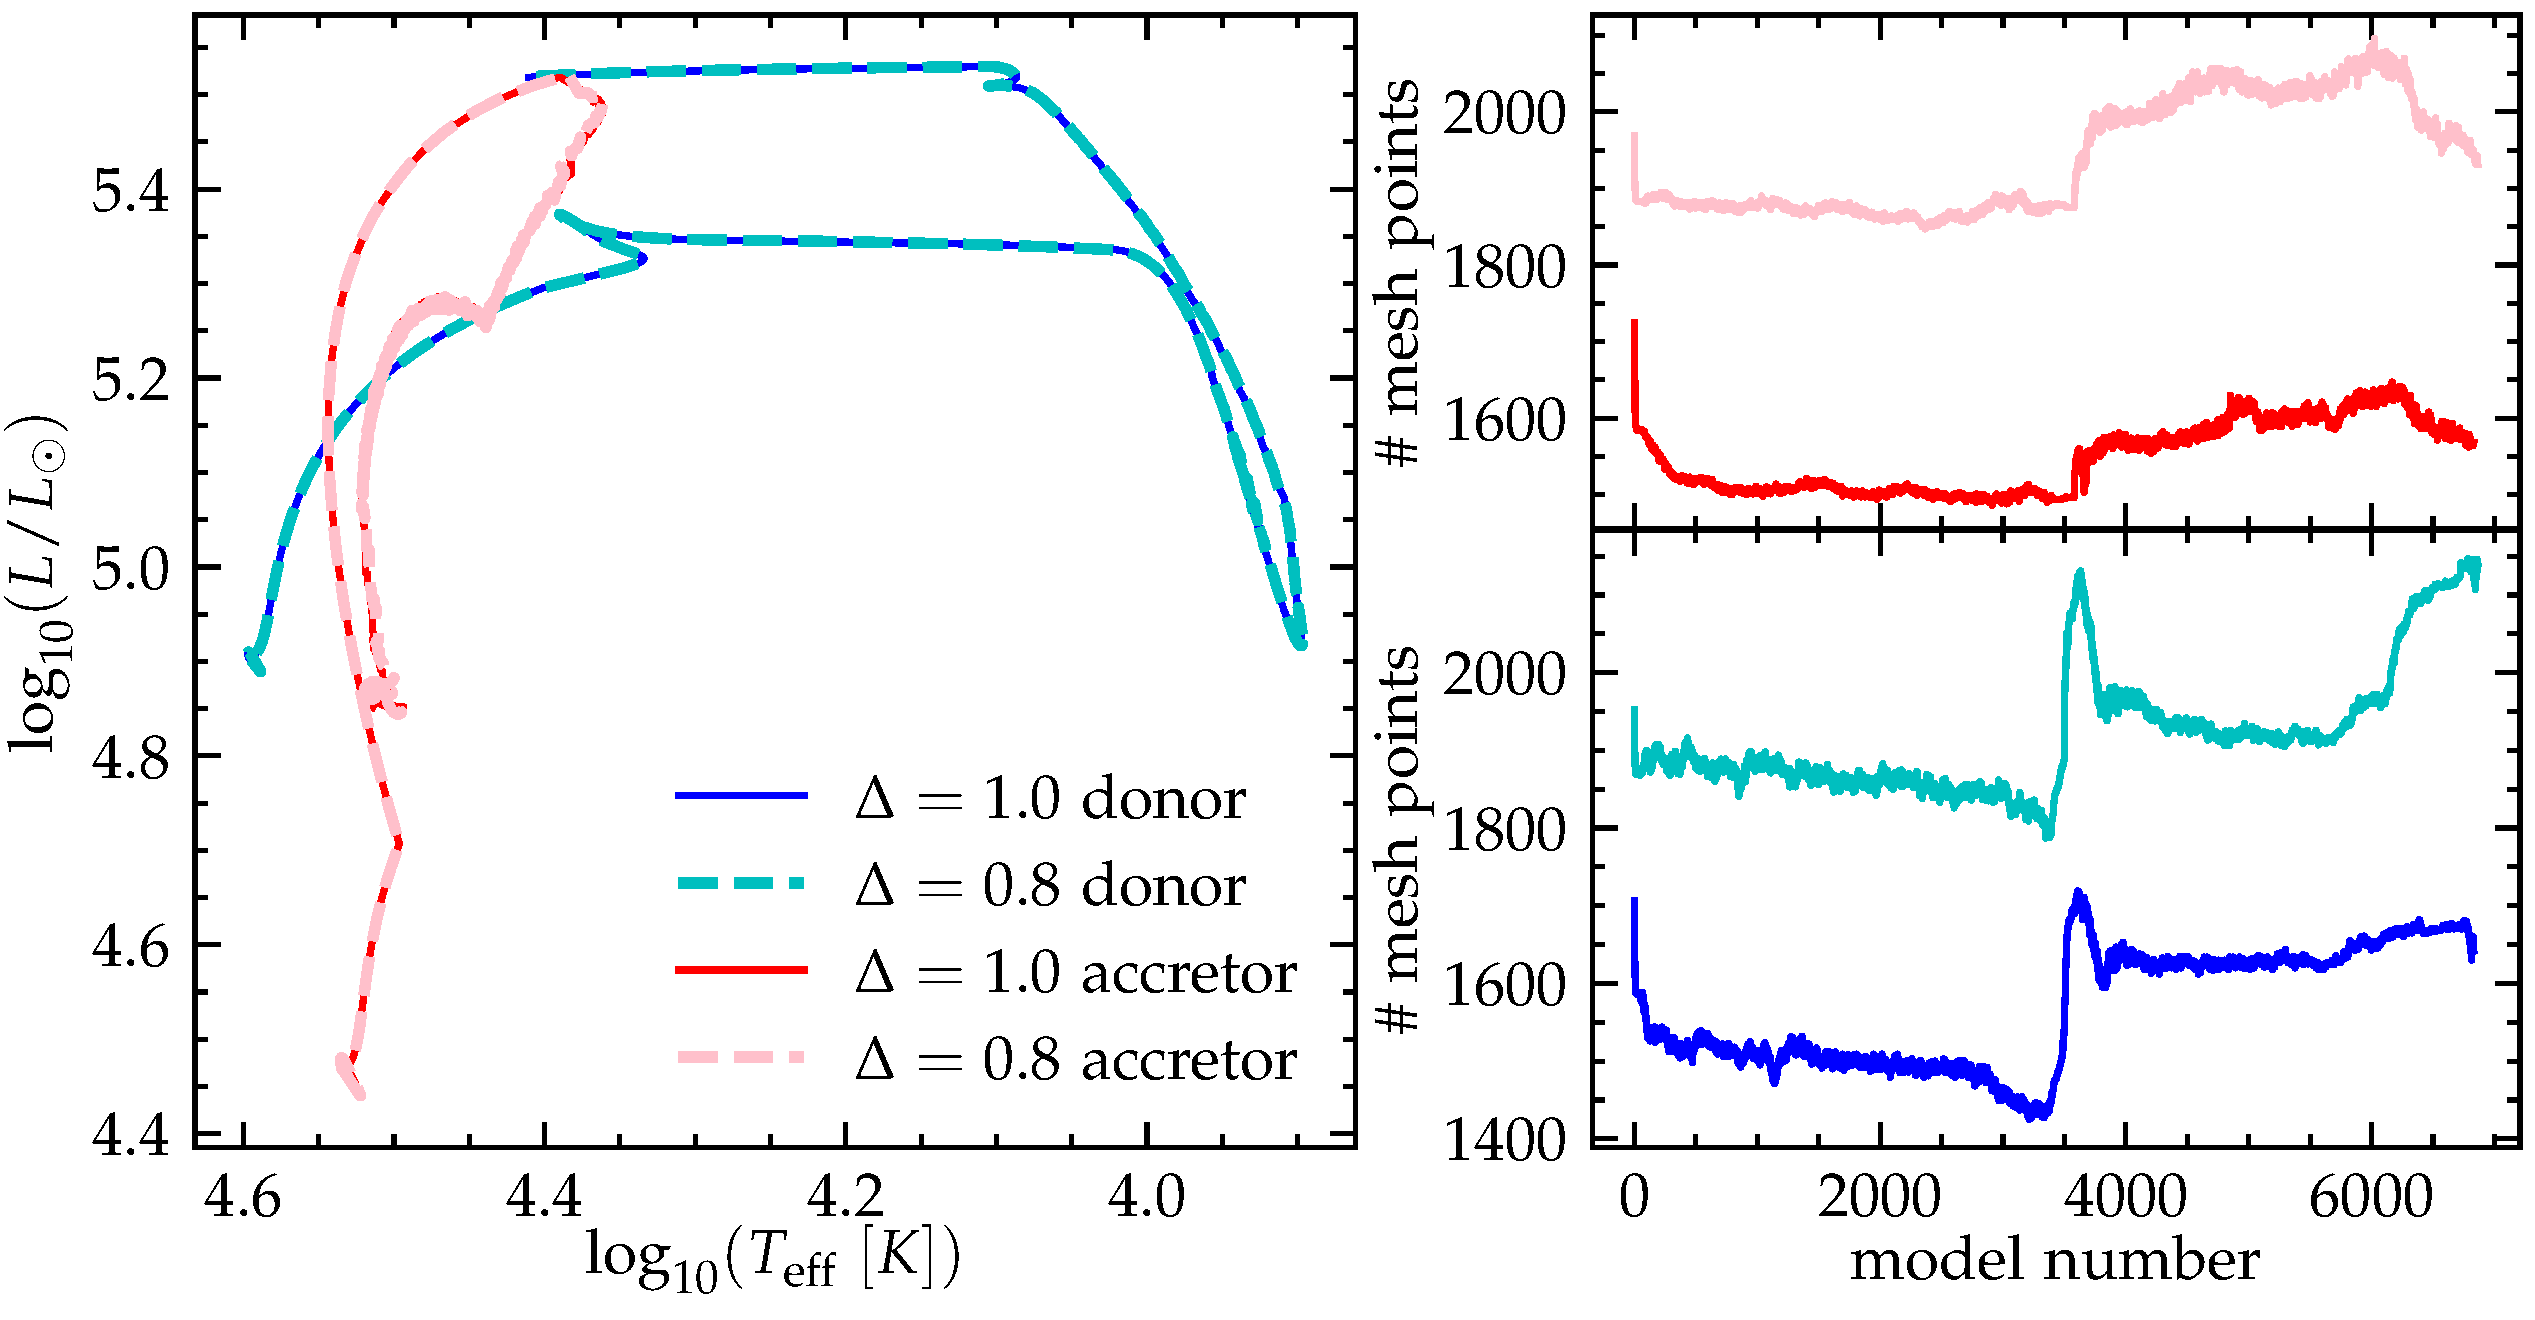
\includegraphics[width=\textwidth]{spatial_res_plot}
  \caption{Left: HR diagram comparison for our fiducial binary model varying
  the number of mesh points. We only show the evolution until our definition
  of RLOF detachment. Right: number of mesh points as a
  function of timestep number. In both panels, the blue/cyan tracks show the donor stars, the
red/pink tracks show the accretor. Thicker dashed lines correspond to
the models at higher resolution (i.e., lower $\Delta$ which indicates
the value of \texttt{mesh\_delta\_coeff}).}
\label{fig:sp_test}
\end{figure*}



We extensively checked the numerical convergence of our stellar
evolution calculations with increasing number of mesh
points. \Figref{fig:sp_test} shows that all the main features described
here do not vary when increasing the spatial resolution by increasing
the number of mesh points (i.e.,
decreasing \texttt{mesh\_delta\_coeff}). The right panel shows the
number of mesh points for the accretor (top) and donor (bottom) as a
function of the model number (akin to an arbitrary time
coordinate). About $\sim$7000 \texttt{MESA} models are used to compute
the binary evolution. The higher resolution run has $\sim 20\%$ more
mesh points. The left panel shows the evolution on the HR diagram until the
detachment of the binary for the two accretor models (pink/red) and
the two donor models (blue/cyan).

Similarly, we tested the numerical convergence with decreasing
timestep size. This can be done decreasing the parameter
\texttt{mesh\_time\_coeff}. However, we were unable to successfully
compute models at higher temporal resolution. Partial results show a
good agreement with our fiducial model until \texttt{MESA} becomes
unable to find a satisfying numerical solution to the stellar
structure equations (typically
during RLOF). Lower temporal resolution models showed a similar
qualitative agreement but increased noisiness during the late RLOF
phase. For our fiducial model the adaptive timestep size never exceeds
$10^{3.8}$\,years with typical pre-RLOF timesteps of the order of $10^{3.2}$\,years
and sub-decade (occasionally sub-year) during RLOF. The main factor limiting the timestep
sizes is the change of surface angular momentum in both stars during
the mass transfer.


\section{Internal composition profile evolution}
\label{sec:X_fig}


\Figref{fig:composition_huge} compares the internal evolution of the composition
profile of single rotating stars with our accretor model.
We show mass fractions of $^{12}\mathrm{C}$  and $^{16}\mathrm{O}$ to complement the
mass fraction of $^{14}\mathrm{N}$ shown in \Figref{fig:n14}, and
reproduced also in the middle panel of \Figref{fig:composition_huge}.


\begin{figure*}[htbp]
  \centering
  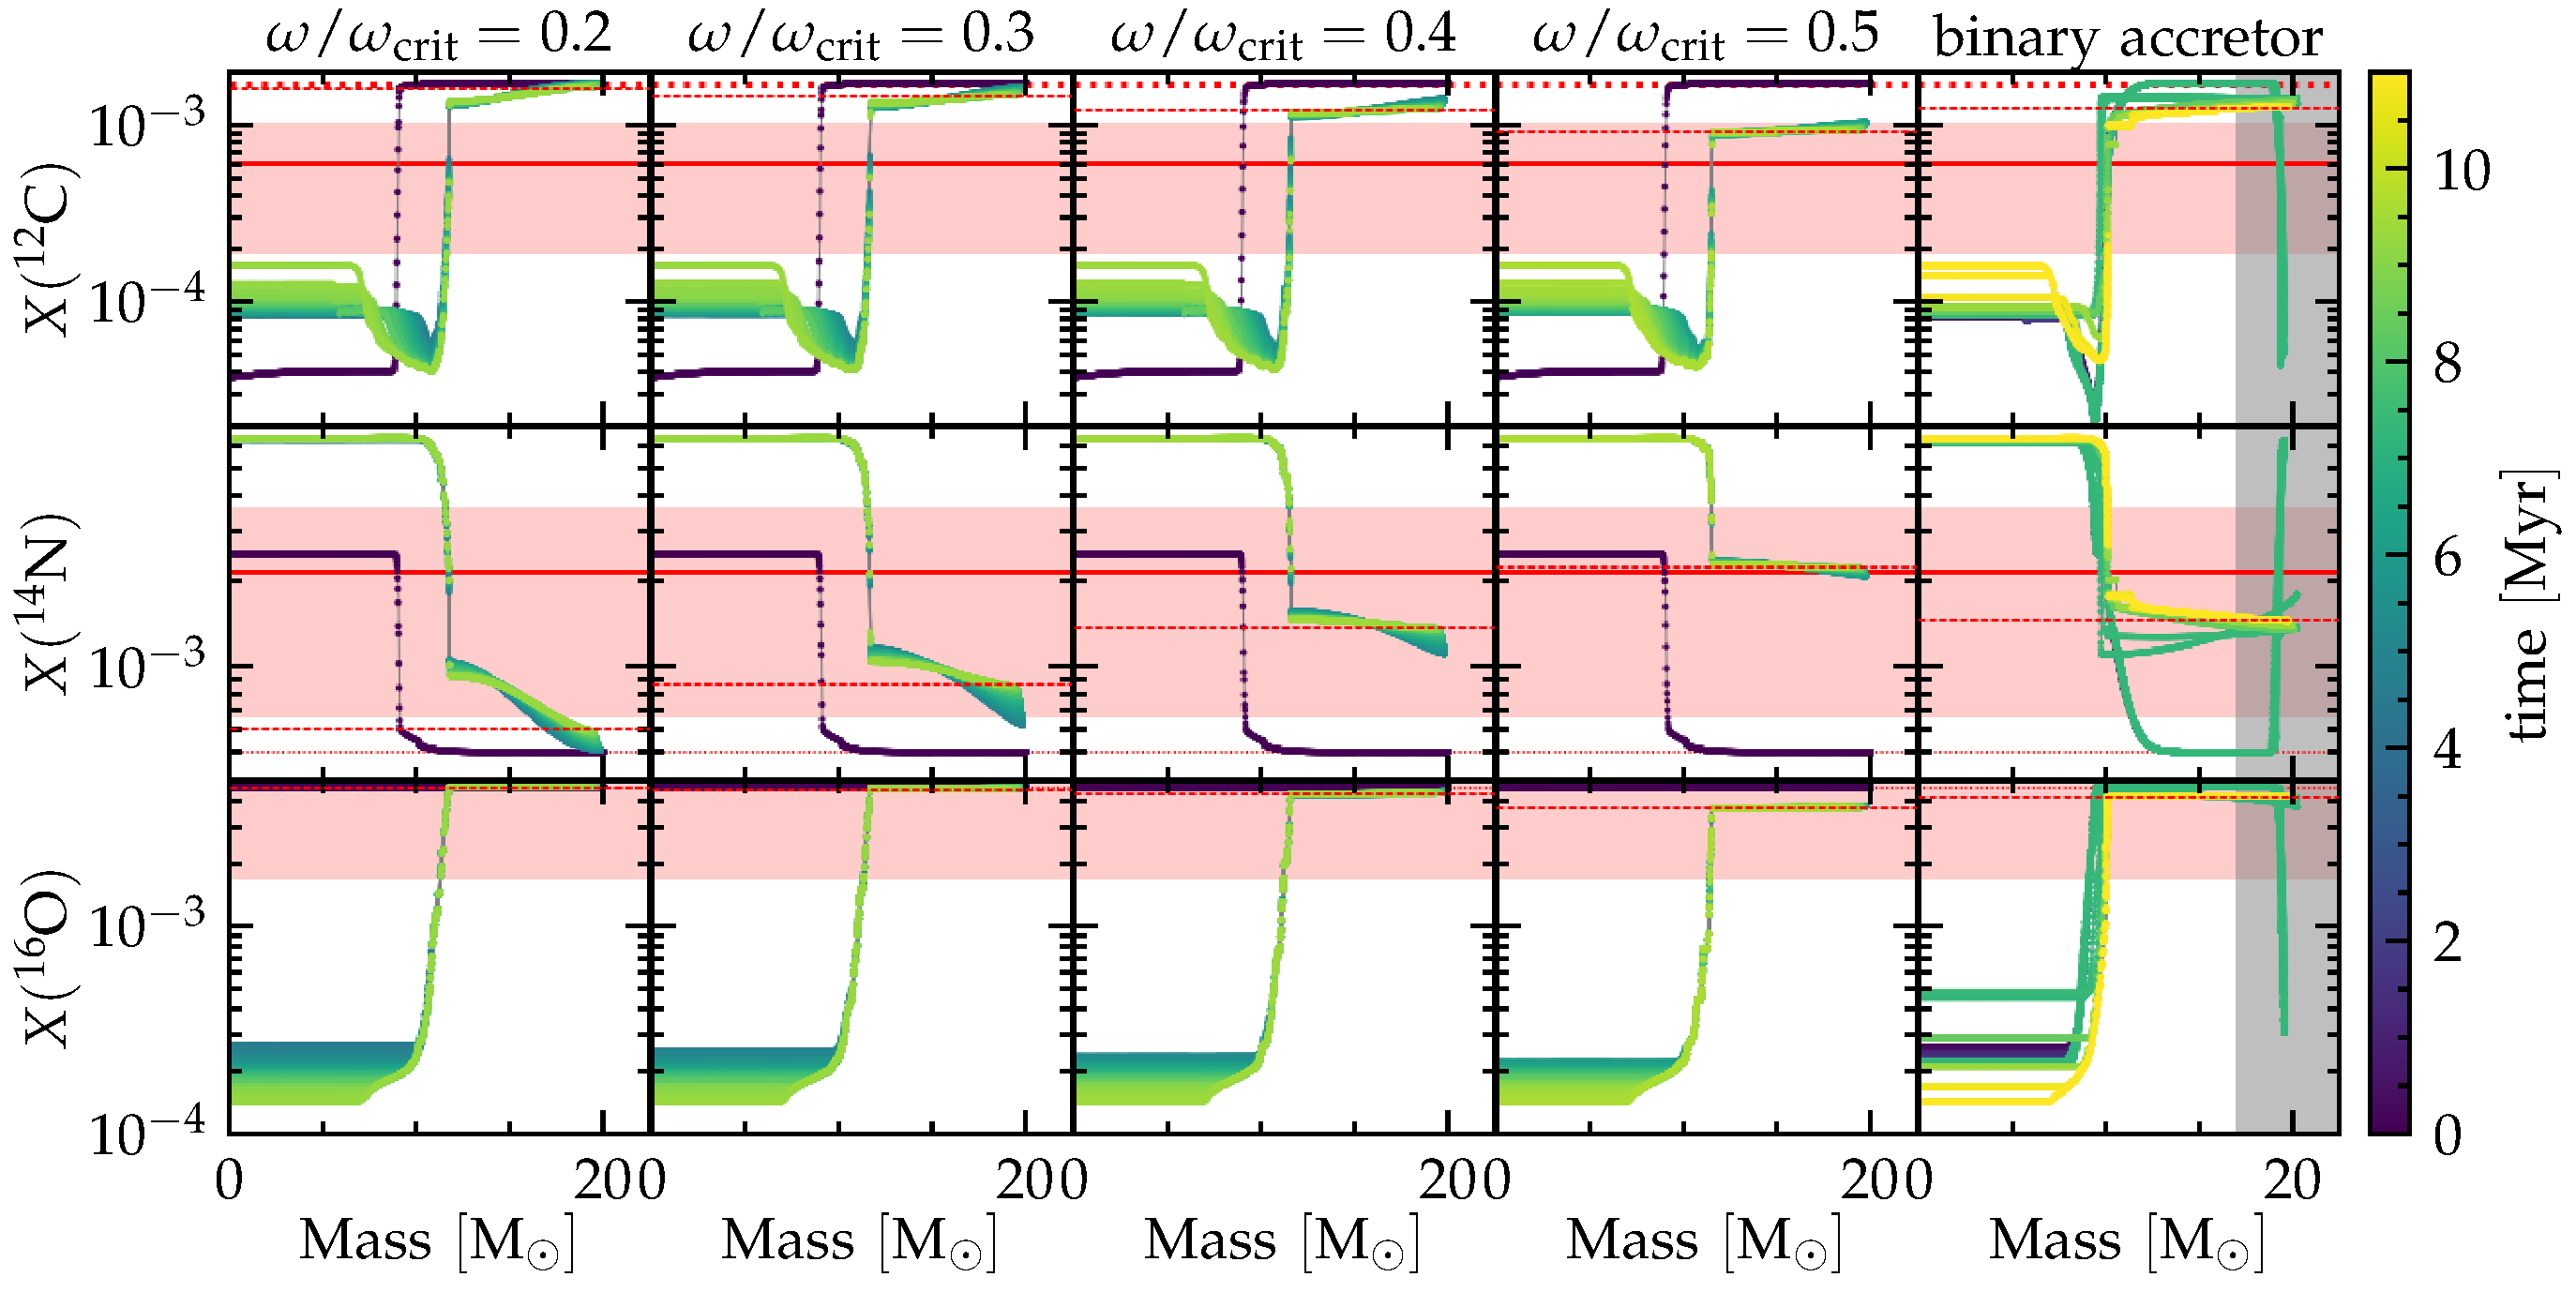
\includegraphics[width=\textwidth]{huge_composition}
  \caption{Same as \Figref{fig:n14}, but for $^{12}\mathrm{C}$ (top
    panel), and $^{16}\mathrm{O}$ (bottom panel). The first four
    panels show single rotating stars of initially $20\,M_\odot$, the
    rightmost panel shows the accretor in our fiducial binary. The middle panel is
    exactly the same as \Figref{fig:n14}. Thick red dotted lines mark the
    initial mass fractions, thin red dashed lines the TAMS surface mass
    fraction, the solid red lines and the semi-transparent red bands
    correspond to the values inferred by \citetalias{villamariz:05}
    using the surface H mass fraction from our model. The tracks go
    from dark (roughly corresponding to ZAMS) to light colors, with the
    lightest color corresponds to TAMS.}
  \label{fig:composition_huge}
\end{figure*}

\bibliographystyle{aasjournal}
\bibliography{./zeta_ophiuchi.bib}


\end{document}

%%% Local Variables:
%%% mode: latex
%%% TeX-master: t
%%% End:
